\chapter{Pattern Recognition and Implementation}

% **************************** Define Graphics Path **************************

\epstopdfsetup{outdir=Chapter4/Figs/PDF/}
\ifpdf
    \graphicspath{{Chapter4/Figs/Raster/}{Chapter4/Figs/PDF/}{Chapter4/Figs/}}
\else
    \graphicspath{{Chapter4/Figs/Vector/}{Chapter4/Figs/}}
\fi


\section{Implementing the Color Space}\label{sec:ImplementingTheColorSpace}

In the previous two chapters, we have been approaching the color space design problem mathematically. Here, we will outline the practical implementation of the color space algorithm on the mobile device.

The first and most pressing consideration is limited processing power; while our mathematical approach to the algorithm design is significantly faster and more efficient than the more typical applications with commonly-used color spaces --- as will be discussed later in this chapter --- minimizing the number of clock cycles spent on continuous processes is necessary in order to ensure efficient operation. In the case of redistribution, the integer matrix transform is performed first, which puts the pixel values in the quantized working type qRsRange described in Chapter 2, then pixel classification is performed before any of the chromatic information is redistributed as illustrated in Figure \ref{fig:PartitioningRegions}.

The pixel classification is performed before the redistribution because it excludes processing pixels which are of no interest based on both chromatic channels, whereas for redistribution one channel may clearly lie outside of the discard region $\lambda$ while the other could be kept or redistributed. With the pixel classifier, if one channel lies outside the discard region, the other is also of no interest since the pixel value is outside of the partitioning region, thereby avoiding unnecessary processing time spent on redistribution. The classification is straightforward within the limits on the channel values, so it isn't sophisticated like an elliptical partitioning or a probabilistic Gaussian-based thresholding; it is simply a quick way of excluding the majority of the pixel values which aren't of interest.

Once the pixels have been classified, the redistribution is performed --- which requires further processing --- or we assign a pixel value from a small set of possibilities and skip onto the next pixel values. The redistribution function is applied to the working type tRange, while the comparison and classification is done in qRsRange. This is because the information in tRange is compressed to avoid wasting space, and as a consequence of this it does not occupy the full data type. qRsRange, on the other hand, being the natural range multiplied by the quantization matrix qR, does occupy the full data type. Since the operation is simply a comparison between numbers, it is of no advantage to compress the information so tightly. Additionally, since qRsRange is a signed range, one could look at the bit indicating the sign and immediately tell whether or not a given value will be discarded. Once scaled to tRange, the redistribution function is applied --- which has a source range of tRange and a range dRange of the destination type --- as outlined in Section \ref{sec:PreservationOfColorInformation} in Chapter 2.

It should be noted that the region between the extended keep region and $\lambda$ is not especially large; for even a $5\sigma$ result, it's only tens of values wide, let alone hundreds. As such, we use a lookup table for the redistribution in our actual implementation, thus further reducing the processing overhead. It should also be noted that C++ has a lookup table threshold set to approximately 64, which makes up a quarter of a region in our case. If the redistribution region is larger than that, the error function approximation from Chapter 2 is implemented. This is mainly for future-proofing the implementation, however; given the limited size of the region, we fully expect to use a lookup table for all practical cases.

As another future concession, the facility to add pixel-based functions to the color space transform, such as the skin probability function mentioned at the end of the previous chapter, is allowed. The color space transform is a threaded process, so there is no way of knowing that the last pixel value that was processed by any given thread was an adjacent pixels, as the parallelization is handled by OpenCV's universal threading library implementations. Pixel-based functions, however, are per-pixel processes, and they come out as separate resulting channels, so they can be added to the color space transform without causing any conflicts.



\subsection{The White-Out Black-Out Algorithm}\label{sec:WhiteOutBlackOutAlgorithm}
We need to find the point at which a chromatic value begins to suffer from white-out and black-out. This is done by taking the corresponding RGB value for the chromatic point and illuminating and deluminating the point by shifting the channel values by the same amount, noting when each channel value becomes fully saturated or desaturated. This is done in the unit space so the results can be scaled to any working range. The algorithm for finding the theoretical values is given in algorithm \ref{algo:TheWhiteoutBlackoutAlgorithm}. 

\begin{algorithm}[H]
 \begin{algorithmic}
  \Require{ $Ca$, $Cb$ The chromatic values}
  \State \phantom{Require}  { $iLCaCb$ the transform to LCaCb from RGB; }
  \State \phantom{Require}  {  $LCaCb$ the transform to RGB from LCaCb}
 \Ensure{  The luminosity at which black out $L_{BO}$  and white out $L_{WO}$ occur.}
 \State \phantom{Ensu} { \begin{tabular}{l}
 $Ca_{min}  \le Ca \le Ca_{max}$   \\ 
 $Cb_{min}  \le Cb \le Cb_{max}$  
 \end{tabular}  \parbox{0.65 \textwidth}{The chromatic range which could be suffering from white-out or black-out}}
 
   \State  $pnt^{RGB} \gets iLCaCb(0.5, Ca,Cb)$ \Comment{Put the point in RGB space }
   \State  $O \gets Order(pnt^{RGB}, \#1> \#2)$ \Comment{The order of the RGB channels from largest to smallest}
   \State  $\Delta WO_1 \gets 1 - pnt^{RGB}_{O(1)} $ \Comment{Iluminate to make the largest channel value saturated}
   \State  \phantom{Set} $pnt^{(RGB, WO, 1)}_{O(1)} \gets 1 $ \Comment{The point where a channel is saturated }
   \State  \phantom{Set} $pnt^{(RGB, WO, 1)}_{O(2)} \gets  pnt^{RGB} _{O(2)} + \Delta WO_1 $ 
   \State  \phantom{Set} $pnt^{(RGB, WO, 1)}_{O(3)} \gets  pnt^{RGB} _{O(3)} + \Delta WO_1 $ 
   \State  $\Delta WO_2 \gets 1 - pnt^{RGB}_{O(2)} $\Comment{Iluminate to make the second largest channel value saturated}
   \State  \phantom{Set}$pnt^{(RGB, WO, 2)}_{O(1)} \gets 1 $ \Comment{The point where two channels are saturated }
   \State  \phantom{Set}$pnt^{(RGB, WO, 2)}_{O(2)} \gets 1 $ 
   \State  \phantom{Set}$pnt^{(RGB, WO, 2)}_{O(3)} \gets  pnt^{RGB} _{O(3)} + \Delta WO_2 $ 
     
     
   \State  $\Delta BO_1 \gets  pnt^{RGB}_{O(3)} $ \Comment{Deluminate by the smallest channel value}
   \State  \phantom{Set}$pnt^{(RGB, BO, 1)}_{O(1)} \gets  pnt^{RGB} _{O(1)} - \Delta BO_1  $ \Comment{The point where a channel is desaturated }
   \State \phantom{Set} $pnt^{(RGB, BO, 1)}_{O(2)} \gets  pnt^{RGB} _{O(2)} - \Delta BO_1 $ 
   \State \phantom{Set} $pnt^{(RGB, BO, 1)}_{O(3)} \gets  0 $ 
   \State  $\Delta BO_2 \gets pnt^{RGB}_{O(2)} $ \Comment{Deluminate by the second smallest channel value}
   \State  \phantom{Set} $pnt^{(RGB, BO, 2)}_{O(1)} \gets pnt^{RGB} _{O(1)} - \Delta BO_2 $ \Comment{The point where two channels are desaturated }
   \State  \phantom{Set} $pnt^{(RGB, BO, 2)}_{O(2)} \gets 0 $ 
   \State  \phantom{Set} $pnt^{(RGB, BO, 2)}_{O(3)} \gets 0 $ 
     
   \State  $pnt^{(WO, i)}\gets LCaCb(pnt^{(WO, i)}) $ \Comment{The white-out points in LCaCb color space}
   \State  $pnt^{(BO, i)}\gets LCaCb(pnt^{(BO, i)}) $ \Comment{The black-out points in LCaCb color space}
   
   \State  $L_{WO} \gets pnt^{(WO, 1)}_1$ 
   \State  $L_{BO} \gets pnt^{(BO, 1)}_1$ 
   \State  $Ca_{min}  \gets Min(pnt^{(WO, 1)}_2, pnt^{(WO, 2)}_2, pnt^{(BO, 1)}_2, pnt^{(BO, 2)}_2 )$ 
   \State  $Ca_{max} \gets Max(pnt^{(WO, 1)}_2, pnt^{(WO, 2)}_2, pnt^{(BO, 1)}_2, pnt^{(BO, 2)}_2 )$ 
   \State  $Cb_{min}  \gets Min(pnt^{(WO, 1)}_3, pnt^{(WO, 2)}_3, pnt^{(BO, 1)}_3, pnt^{(BO, 2)}_3 )$ 
   \State  $Cb_{max} \gets Max(pnt^{(WO, 1)}_3, pnt^{(WO, 2)}_3, pnt^{(BO, 1)}_3, pnt^{(BO, 2)}_3 )$ 
     
  \State \textbf{Return} {$L_{WO} , L_{BO} , Ca_{min}, Ca_{max} , Cb_{min}, Cb_{max}$ }
 
  \end{algorithmic}
    \caption{The White-Out Black-Out Algorithm}
    \label{algo:TheWhiteoutBlackoutAlgorithm}
 \end{algorithm}
 
 The theoretical values are adjusted by 10\% to account for the auto brightness and contrast adjustment performed by the phone as described in Chapter 3, Section \ref{sec:WhiteoutAndBlackout}. We only wish to adjust the bounds away from the luminosity axis. One of the chromatic bounds will be the luminosity axis $Ca=\frac{1}{2}$ or  $Cb=\frac{1}{2}$, as this is the white or black point. Whether the bound is the upper or lower limit depends on the starting point, so we define a function which performs the adjustment appropriately.
 
 \begin{equation}
 slack(x) = \begin{cases}
 (1-a) x     & x < \frac{1}{2} \\
 (1+a) x     & x > \frac{1}{2} \\
 \frac{1}{2} & x = \frac{1}{2} 
 \end{cases} \quad \text{where} \quad a = 0.1
   \end{equation}
 We can now write the condition for whether a value could have suffered from white-out or black-out. 
  \begin{multline}\label{eq:InWoBoRegion}
 (( 0 \le L \le  slack(L_{BO}) ) \vee ( slack(L_{WO}) \le L \le 1) ) \wedge  \\
 slack(Ca_{min}) \le Ca \le  slack(Ca_{max}) \wedge  \\
 slack(Cb_{min}) \le Cb \le  slack(Cb_{max})
  \end{multline}
  
  \subsection{The Region Classification and Partitioning Function}\label{sec:TheRegionClassificationAndPartitioningFunction}
  It is desirable to classify a pixel value after rotation but before redistribution, using channel limits by how well the value fits the target and by how reliable the value is given lighting conditions. This can be done to a degree, but it is necessary to assume reasonably uniform lighting conditions. The pixel values are classified by chromatic value as either inside the target region or outside in both axes, dividing the chromatic plane into nine regions, as illustrated in Fig \ref{fig:PartitioningRegions}. A rudimentary partitioning is performed by assigning 8 constants to the values outside the region around the mean. The luminosity is always evaluated, because all that is required is a scaling from qRsRange to the destination range dRange. 
  
  \begin{figure}[h!]
    \centering
      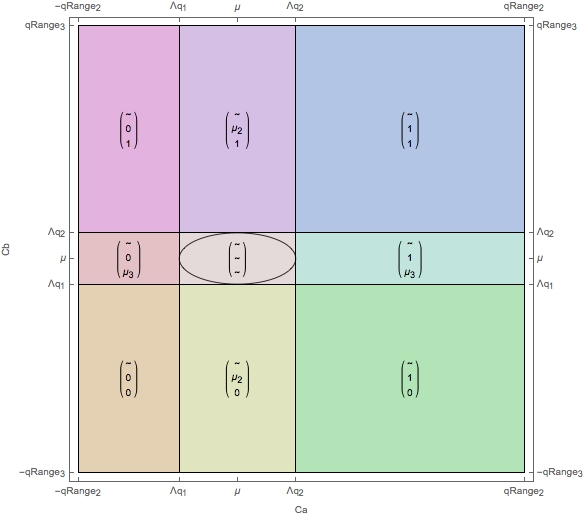
\includegraphics[width=0.80\textwidth]{Chapter4/Figs/PartitioningRegion.jpg}
      \caption{The Regions in the chromatic space. ~ Indicates values which will undergo redistribution. Regions outside the target area are allocated extreme values at the edge of the color space}  \label{fig:PartitioningRegions}
  \end{figure}
  
  
  
  \subsection{Floating the Mean}\label{sec:FloatingTheMean}
  Different lighting conditions can affect the detected pixel color. Not accounting for strongly-colored light, the affect of different lighting conditions is to increase or decrease the saturation of the color. The distribution is relatively unaffected in orientation or variance, meaning that lighting conditions can be accounted for by adjusting the mean. 
  \newcommand{\newMean}{\widetilde{\mu}}
  The algorithm adjusts to ambient lighting by first taking a reference image centered on a patch of skin and finding the mean in the LCaCb color space. This new mean $\newMean$ is then used in the current instance of the algorithm. It is adventitious to keep the mean adjustable in the routine, so this is implemented by introducing an adjustment parameter $\delta\mu$ to the routine, where $\newMean = \mu + \delta\mu$. The algorithm assumes that the adjustment is small enough that the distribution function retains the same shape aside from a translation along the axis. This allows the distribution parameters to be adjusted by simply shifting them by $\delta\mu$. 
  
  \begin{equation}
  \begin{aligned}
   \widetilde{\lambda}_1 & = \lambda_1 + \delta\mu &  \widetilde{\lambda}_2 & = \lambda_2 + \delta\mu \\
   \widetilde{\omega}_1 & = \omega_1 + \delta\mu &  \widetilde{\omega}_2 & = \omega_2 + \delta\mu 
  \end{aligned} \quad \text{Where} \quad \lambda_1 < \delta\mu < 1 - \lambda_2
  \end{equation}
  
  \subsection{Loosened Deviation}\label{sec:LoosenedDeviation}
  
 \afterpage{ \begin{figure}[h!]
    \centering
      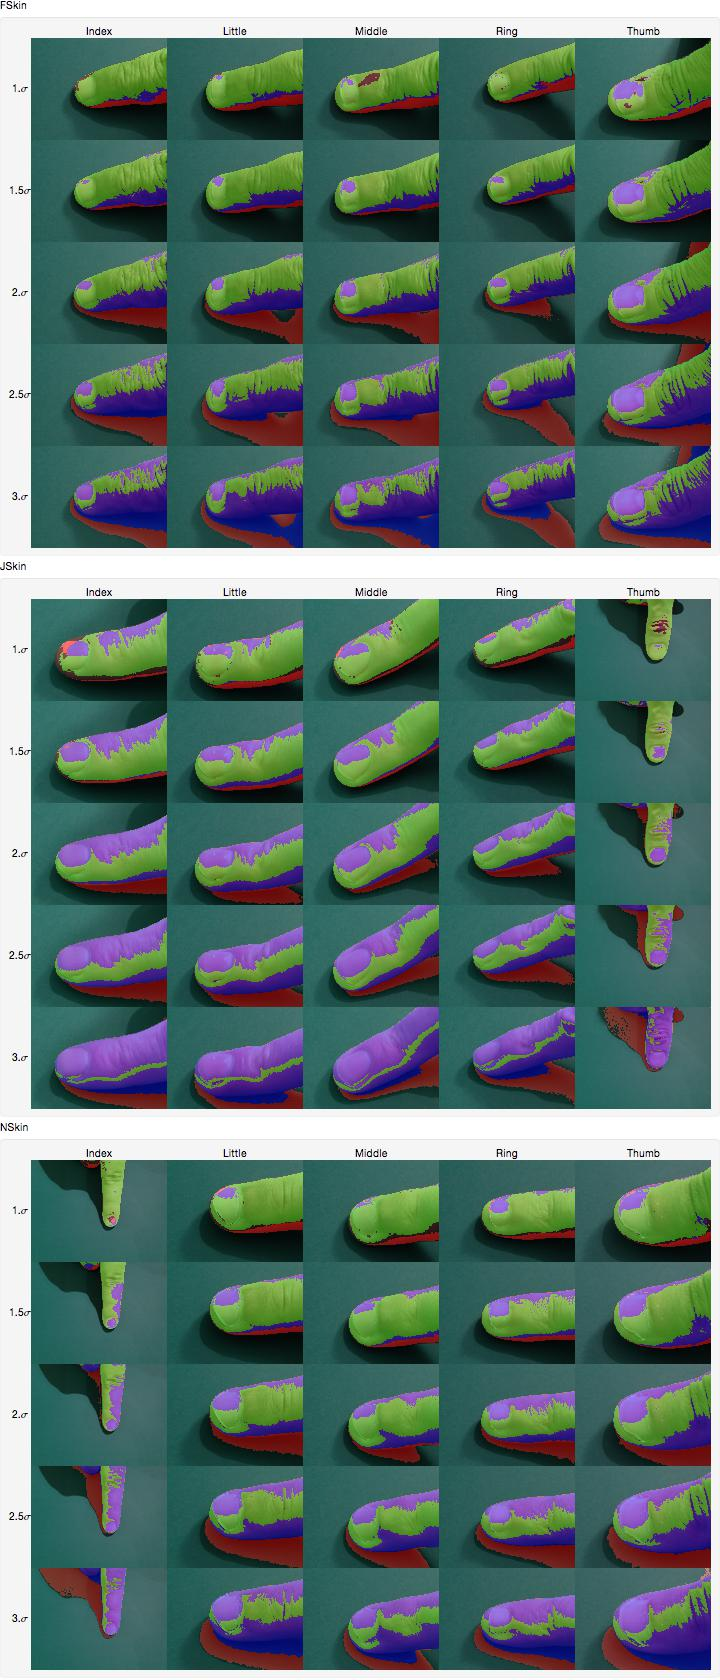
\includegraphics[width=0.85\textwidth,height = \textheight]{Chapter4/Figs/RelaxingSigma.jpg}
      \caption{A selection of images classified using the trinary method outlined in section <so-and-so>, with various values of $\sigma$. It can be seen that $1\sigma$ correctly classifies the majority of pixels, however it classifies some on-digit pixels as "probably not skin", and even "not skin". $3\sigma$, meanwhile, includes large portions of shadow as "probably skin". A compromise of $2\sigma$-$2.5\sigma$ is therefore suggested.} \label{fig:RelaxedSigma}
  \end{figure}
  \clearpage
  }
  
  The standard deviation found in Chapter 3 is a very tight fit to the chromatic values taken under controlled lighting conditions. For our practical implementation, this tight fit needs to be relaxed. This is done empirically by trying out multipliers of the standard deviation $\sigma$ on the image sets. What is desired is a multiplier which relaxes the redistribution such that all the pixel values on a given digit are classified as skin, and all the background is classified as not skin. This is done empirically using the trinary classification presented below (in section <so-and-so>), which accounts for white-out and black-out and classifies the pixel value as "definitely skin", "probably skin", "probably not skin", and "not skin".
  
  Using a value of 2.3 times the original $\sigma$ correctly classifies the pixel values; this was found by observing tables of images similar to those in Figure \ref{fig:2BitImage}. 
  
  
  \subsection{The Color Space Algorithm as Implemented}\label{sec:ColorSpaceAlgorithmAsImplemented}
  Here we present the color space algorithm in a way which most closely resembles the C++ code. The construction of the color space object is described at the end of Chapter 2; here, the operation of the algorithm is described.
  
  First, we determine the form of the distribution function for a working type tRange with the source range $srcRange=2^n$  and destination range $dstRange=2^m$ expressed in terms of their bit depths.
  
  \begin{gather*}
  \begin{aligned}
  K & =  2^{m-n}  \quad & \quad  
  \tRange(\theta,\mu,\sigma)   & =  \mathbf{l} \; 2^n \quad & \quad
  \mathbf{l}  & = \min\left\{ 2^{m-n}\delta(\mu,\sigma) \right. ,  \left. \mathbf{L}(\theta) \right\} 
   \end{aligned} \\
   \begin{aligned}
    \tMin(\theta,\mu,\sigma)   & =
   \begin{pmatrix}
      0 \\
    -\mathbf{l}_2 \; 2^{n-1}  \\  
    -\mathbf{l}_3 \; 2^{n-1} \\  
   \end{pmatrix} \quad & \quad
    \tMax(\theta,\mu,\sigma)   & =
   \begin{pmatrix}
    \mathbf{l}_1 \; 2^n  \\
    \mathbf{l}_2 \; 2^{n-1}  \\  
    \mathbf{l}_3 \; 2^{n-1} \\  
   \end{pmatrix} \quad & \quad
     \Scale &=
      \mathbf{l} \otimes
     \begin{pmatrix}
       \frac{1}{3} \\
      2^{1-n } \\
      2^{1-n }  \\
     \end{pmatrix}    \\
   \end{aligned}
  \end{gather*}
  
  Substituting into the distribution function \ref{eq:disFunction} gives us
  
  \begin{equation}
\textbf{dis}(x) =  -\frac{2^n \left(\text{erf}\left(\frac{2 \mu +1}{2 \sqrt{2} \sigma }\right)+\text{erf}\left(\frac{2^{1-2 n} x-\mu }{\sqrt{2} \sigma }\right)\right)}{\text{erf}\left(\frac{2 \mu -1}{2 \sqrt{2} \sigma }\right)-\text{erf}\left(\frac{2 \mu +1}{2 \sqrt{2} \sigma }\right)} \quad \textbf{where} \quad
\begin{array}{rl}
qMin < & x  < qMax \\
0 < &\mu <1\\
0 < &\sigma <1
\end{array}
  \end{equation}
  
  This form takes the result of the rotation directly, however we wish to add the flexibility to adjust the mean and use a lookup table for the values. It is desirable to keep the lookup table as short as possible. The maximum compression of the information without losing relevant information is given by compressing to tRange. The number of values in the lookup table can be reduced by scaling $x$ by a range qtRange, which is chosen to balance lookup table size and computational scaling efficiency.  Noting that $\mathbf{l} <2$, qRsRange can be chosen to be equal to tRange as if $\mathbf{l} =2$, which means that qtRange is a power of two, allowing the scaling to be performed by bit shifting the value of $x_{qt} = x \ll n-2$. However, in the region where the function is applied, the information is preserved at best 2-to-1, so the information density can be reduced by half $x_{qt} = x \ll n-1$. Adjusting the mean changes the bounds on the region to be redistributed such that the form of the function does not change. For this reason, we also define $x$ relative to the bounds, which allows the same lookup table to be used regardless of any adjustment to the mean.
  
    \begin{equation}
  \textbf{dis}(x) =  \begin{cases}
    \textbf{disLU}((x-\Lambda_{1}) qtRange)  & \Lambda_{1} < x < \Omega_{pq1} \\
  \textbf{disLU}((x-\Omega_{pq2}) qtRange)  & \Omega_{pq2} < x < \Lambda_{q2} \\
  \textbf{dis}(x)  & \text{Otherwise}
    \end{cases} \quad \text{where} \quad 
    qtRange = \left(\begin{smallmatrix}
    \cdots \\ 2^{1-n}\\2^{1-n}
    \end{smallmatrix}\right)
    \end{equation}
  
  Aside from these refinements, the algorithm presented in Chapter 2 is used to perform the rotation and redistribution as described. The algorithm proceeds as follows:
  
  \begin{itemize}
  \item Interactively find an adjustment to the mean  $\delta\mu$. .
  \item Set the new distribution parameters
  \item Rotate the pixel value with the $\qR$ matrix. $ pxl_{q} = \qR \cdot pxl_{RGB}$ then $ \frac{- qRsRange}{2} < pxl_{q} < \frac{ qRsRange}{2}$
  \item Partition the rotated values to avoid unnecessary processing of irrelevant information.
  \item Apply any user supplied per-pixel functions to the rotated value and add as extra channels.
  \item Redistribute the rotated values into the destination type.
  \item Apply and user supplied per-pixel functions to the redistributed values.
  \end{itemize}

\section{Pattern Recognition Routines}\label{sec:PatternRecognitionRoutines}
In this section, pattern recognition routines which use the new color space are presented and discussed.

\subsection{Trinary Pixel Classification}\label{sec:TrinaryPixelClassification}

\newcommand{\WoBoBool}{\underset{\scalebox{0.5}{WoBo}}{\mathbb{L}}}
\newcommand{\ColorSquareBool}{\underset{ \scalebox{0.5}[0.5]{square} }{ \mathbb{C} } }
\newcommand{\ColorEllipseBool}{\underset{ \scalebox{0.5}[0.5]{ellipse} }{ \mathbb{C} } }

OpenCV's findContours method takes a binary image and finds the contours in that binary image. However, the problem with this method is that we're thresholding on chromatic values, i.e. using color information to break up the image into blobs in which we're finding the contours. This doesn't take into account the white-out and black-out, which was noted previously. This is done by applying equation \ref{eq:InWoBoRegion} and setting a boolean flag $\WoBoBool$ accordingly. The square partitioning performed earlier in the algorithm also sets a boolean flag $\ColorSquareBool$ to 1 if the pixel is within the target range and to 0 otherwise. These can be combined to produce a 2-bit image which indicates both if the pixel value is in the target chromatic range and the reliability of the classification.
% 

\begin{center}
\begin{tabular}{|c|c|c|c|c|}
\hline
Correct                               & Unreliable      & \multicolumn{2}{|c|}{Image Bit} & \multicolumn{1}{|c|}{\multirow{2}{*}{Comment}}  \\ \cline{1-4}
Color $\ColorSquareBool$ & $\WoBoBool$ & $\ColorSquareBool$ & XOR($\ColorSquareBool$, $\WoBoBool$) & \\\hline
0 & 0 & 0 & 0 &  Definitely not the target \\\hline % & Wrong Color &    Reliable Luminosity 
0 & 1 & 0 & 1  & Possibly the target but shifted. \\\hline % & Wrong Color & Unreliable Luminosity
1 & 1 & 1 & 0  & \begin{tabular}{l} Probably the target but possibly \\ shifted into the target region \end{tabular} \\\hline % &   Right Color &    Reliable Luminosity
1 & 0 & 1 & 1  & Definitely the target \\\hline % &   Right Color & Unreliable Luminosity
\end{tabular}
\end{center}


This produces a 2-bit image. For this purpose, a 2-bit data type was added to OpenCV. The question then is how to use it. Essentially, we have four different states: values which are neither the right color nor in the right region; values which are possibly the right color, but because they're outside the valid region, they've potentially suffered from white-out and black-out and as such they are not reliable indicators for either the start of an edge or the end of an edge; values which are in the right region, but the wrong color, and we are certain that they are not skin; and finally, values which are in the valid region and are of the right color.

The Canny edge detector method is perfect for implementing a decision by setting a high threshold --- our strong criteria --- in the right region in the right color, and a low threshold so that it will continue following an edge across values which are in the invalid region. Whichever value we set the low threshold to depends on the state of the image; we use a lower value if there is ambiguity and a higher value if the result is fairly accurate:
 
\begin{figure}[h!]
  \centering
    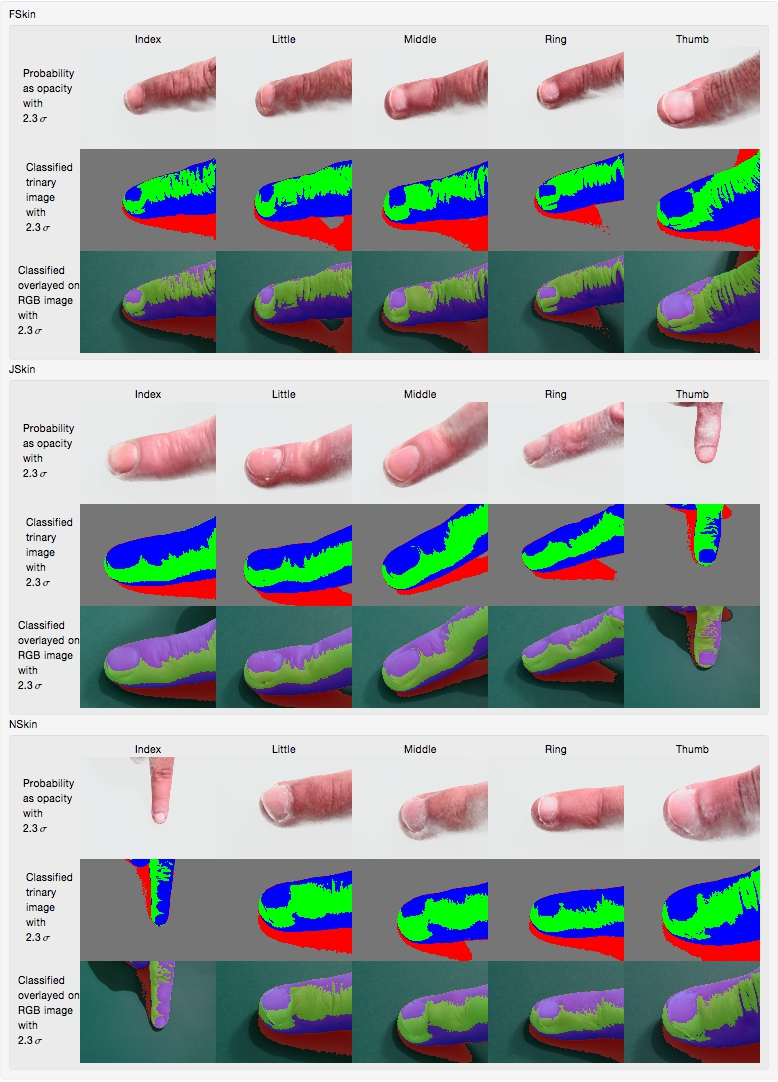
\includegraphics[width=0.95\textwidth]{Chapter4/Figs/ClassifiedSkin.jpg}
    \caption{The Pixel Classification.}\label{fig:2BitImage}
\end{figure}

\subsection{The 'Hurdle' Method}\label{sec:HurdleMethod}
The Hurdle method is an algorithm for finding a path inside an object using the trinary classified image. The Hurdle method follows straight line paths in the object. As written, it is flexible enough to follow any straight line, however the current implementation takes a direction vector and evaluates at multiples of that direction vector. This means that non-horizontal and non-vertical lines are not guaranteed to be continuous. This is because the pixel values are not found using Bresenham's line algorithm. The algorithm has two thresholds --- a high and a low threshold. Whilst the pixel values remain in the high threshold, the path end point variable is updated; when the pixel values are in the lower threshold, the algorithm continues along the path, but without updating the path end point. This allows the path to pass through artifacts (i.e. pixel values which are inside the object but which have been misclassified), but does not allow the path to extend outside of the object into regions which are, for instance, in the shadow of the object.
 
\subsection{The 'Filament Fill' Method}\label{sec:FilamentFill}
The Filament Fill method takes a path --- given as a sequence of points --- within an object and finds the edges of the object using the Hurdle method running away from the path within the object. Assuming a horizontally-oriented object, the path's extent in the horizontal direction is divided equally into points, and these points are used to start the Hurdle method in the vertical directions, and vice versa for vertical-oriented objects.


\begin{figure}[h!]
  \centering
    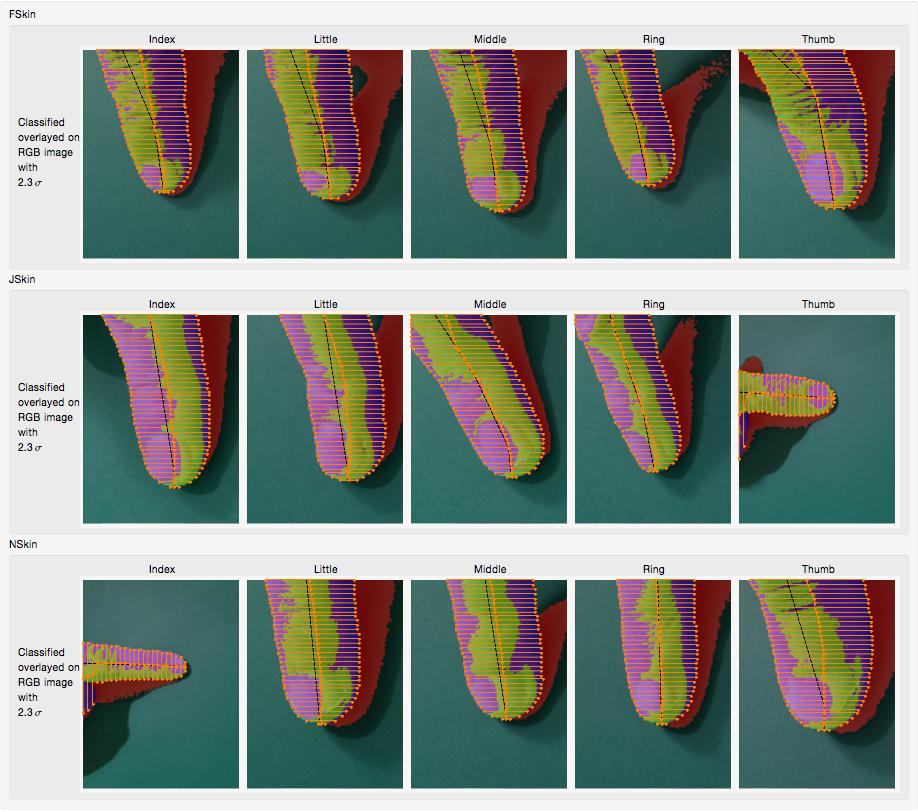
\includegraphics[width=0.95\textwidth]{Chapter4/Figs/FillamentFill.jpg}
    \caption{The 'Filament Fill' Method.}\label{fig:FillamentFill}
\end{figure}

\subsection{The 'Mean-Medians' Method}\label{sec:MeanMedians}
For the purposes of the shape detection algorithms, there are metrics that are applied which suffer from noise and anomalies, where the noise is due to the natural variability of human digits from regular geometric forms, and the anomalies are due to misdetections of the edges of the digit. We assume that the anomalous results are extreme values, however we acknowledge that the most common (mode) or middle (median) values may not be representative of the best geometric approximation for the shape. The Mean-Median method --- similar the "k-Nearest Neighbors" algorithm --- solves this problem by taking a confidence interval around the median and then taking the mean of the points within this interval. This method is a useful adaptation of methods like the k-Nearest Neighbors in that it solves the outlier problem for this particular application.

\subsection{The 'Kink Fit' Method}\label{sec:KinkFitMethod}
The Kink Fit algorithm takes in a set of 2D points, where the first component is taken to be independent variable and the second component is taken to be the dependent variable. This assumption excludes the possibility of truly vertical lines being presented to the algorithm. The Kink Fit algorithm fits a function which consists of two straight-line segments to a set of points. Unfortunately, currently the only piecewise linear fitting function is the proprietary MARS algorithm which, aside from being commercial, is overkill for this particular problem, which has a small number of points which are well-aligned. 

The Kink Fit algorithm relies on the fact that we know that the points are in order; it chooses a point and divides the set in two, and then performs a standard, least squares linear fit to the two sets. Both sets include the point at which the set is divided. 

The fit is also assumed to be continuous, except in the first derivative. The algorithm as described above may produce two lines which do not intersect between the second-to-last data point used for the first line and the second data point used for the second line. The algorithm needs to ensure that this is the case. This is achieved by shifting the second half of the data set by the end point of the linear fit to the first half of the data set. The point at which the two linear fits intersect is found, and if that point is between the second-to-last point in the first set, and a second point in the second set (i.e. the points on either side of the point of division), then the fit is considered to be acceptable. If the fit is not acceptable, it indicates that there's a discontinuity in position rather than simply being a discontinuity in the first derivative. This is handled by choosing the point on the fit to the first set closest to the intersection within the bounds of the points on either side of the point of division. The linear fit is then performed with only the gradient as the free parameter, guaranteeing that the line will have passed through this limiting point.

The algorithm then finds the residuals, and then finds the average of the square of the residuals. This is considered the score for dividing the set of points at that position. The algorithm finds the point which minimizes the score using a bisecting algorithm; if a linear fit to the data has a low score, then the Kink Fit algorithm is considered unnecessary and the digit is assumed to be in a relaxed, straight, neutral pose. The algorithm specifies a minimum number of points to be included in a set, as this avoids the problem of dividing into sets which contain only one point.

\subsection{The 'Elliptical Fit' Method}\label{sec:EllipticalFitMethod}
Fitting an ellipse to a set of points is surprisingly difficult. The reason for this is as follows:

To follow the standard linear algebra approach to least squares fitting, we need to decide upon a functional form for the fit, and thereby a basis set. For an ellipse, this basis set is $\chi= \left(x^2, x y, y^2, x, y, 1\right)$, which is a set of six free coefficients $ A^T=\left\{A_{\text{xx}},A_{\text{xy}},A_{\text{yy}},A_x,A_y,A_0\right\}$. However, to specify an ellipse, all that is needed is five numbers; the major and minor axes lengths $(a,b)$, the position $(x_0,y_0)$, and the orientation $\theta$. This is because the basis set includes lines, quadratics, parabolic and hyperbolic functions as well as elliptical functions as possible fits. An additional difficulty arises when we try to construct a cost function for an ellipse. Ideally, we wish to minimize the perpendicular distances of the points from the ellipse, but the calculation of the distance of a point from an ellipse is not straightforward, requiring the roots of a fourth degree polynomial to be found. Due to these complexities, several different methods have been proposed by different authors, but we will be focusing on two methods: The Approximate Mean Square (AMS)  proposed by (\cite{Taubin1991}), and the Direct least square (Direct) method by (\cite{Fitzgibbon1999}).


For the fingertip problem, there is also the added difficulty that the points that are confined to one side of the ellipse so we have chosen methods which cope well with partially occluded ellipses. Both methods begin by forming the design matrix and then apply an additional constraint which restricts the fit to a family of curves. Both methods are formulated as generalised eigenvalue problems avoiding the need for iterative methods.

The AMS method restricts the fit to parabolic, hyperbolic and elliptical curves by imposing the condition that $ A^T ( D_x^T D_x  +   D_y^T D_y) A = 1$ where the matrices $Dx$ and $Dy$ are the partial derivatives of the design matrix $D$ with respect to x and y. The matrices are formed row by row applying the following to each of the points in the set:
\begin{align*}
D_x(i,:)&=\left\{x_i^2, x_i y_i, y_i^2, x_i, y_i, 1\right\} &
D_x(i,:)&=\left\{2 x_i,y_i,0,1,0,0\right\} &
D_y(i,:)&=\left\{0,x_i,2 y_i,0,1,0\right\}
\end{align*}
The AMS method minimizes the cost function
\begin{equation*}
\epsilon ^2=\frac{ A^T D^T D A }{ A^T (D_x^T D_x +  D_y^T D_y) A^T }
\end{equation*}

The minimum cost is found by solving the generalized eigenvalue problem.

\begin{equation*}
 D^T D A = \lambda  \left( D_x^T D_x +  D_y^T D_y\right) A 
\end{equation*}

The Direct method confines the fit to ellipses by ensuring that $4 A_{xx} A_{yy}- A_{xy}^2 > 0$. The condition imposed is that $4 A_{xx} A_{yy}- A_{xy}^2=1$ which satisfies the inequality and as the coefficients can be arbitrarily scaled is not overly restrictive.

\begin{equation*}
\epsilon ^2= A^T D^T D A \quad \text{with} \quad A^T C A =1 \quad \text{and} \quad C=\left(\begin{matrix}
 0 & 0  & 2  & 0  & 0  &  0  \\ 
 0 & -1  & 0  & 0  & 0  &  0 \\ 
 2 & 0  & 0  & 0  & 0  &  0 \\ 
 0 & 0  & 0  & 0  & 0  &  0 \\ 
 0 & 0  & 0  & 0  & 0  &  0 \\ 
 0 & 0  & 0  & 0  & 0  &  0 
\end{matrix} \right)
\end{equation*}

The minimum cost is found by solving the generalized eigenvalue problem.

\begin{equation*}
 D^T D A = \lambda  \left( C\right) A 
\end{equation*}

The system produces only one positive eigenvalue $ \lambda$ which is chosen as the solution with its eigenvector $\mathbf{u}$. These are used to find the coefficients

\begin{figure}[p]
\centering
\subfloat[Comparison of the AMS and Direct ellipse fit methods for a complete ellipse][AMS and Direct methods both perform well with a set of points evenly distributed arround the ellipse. ]{
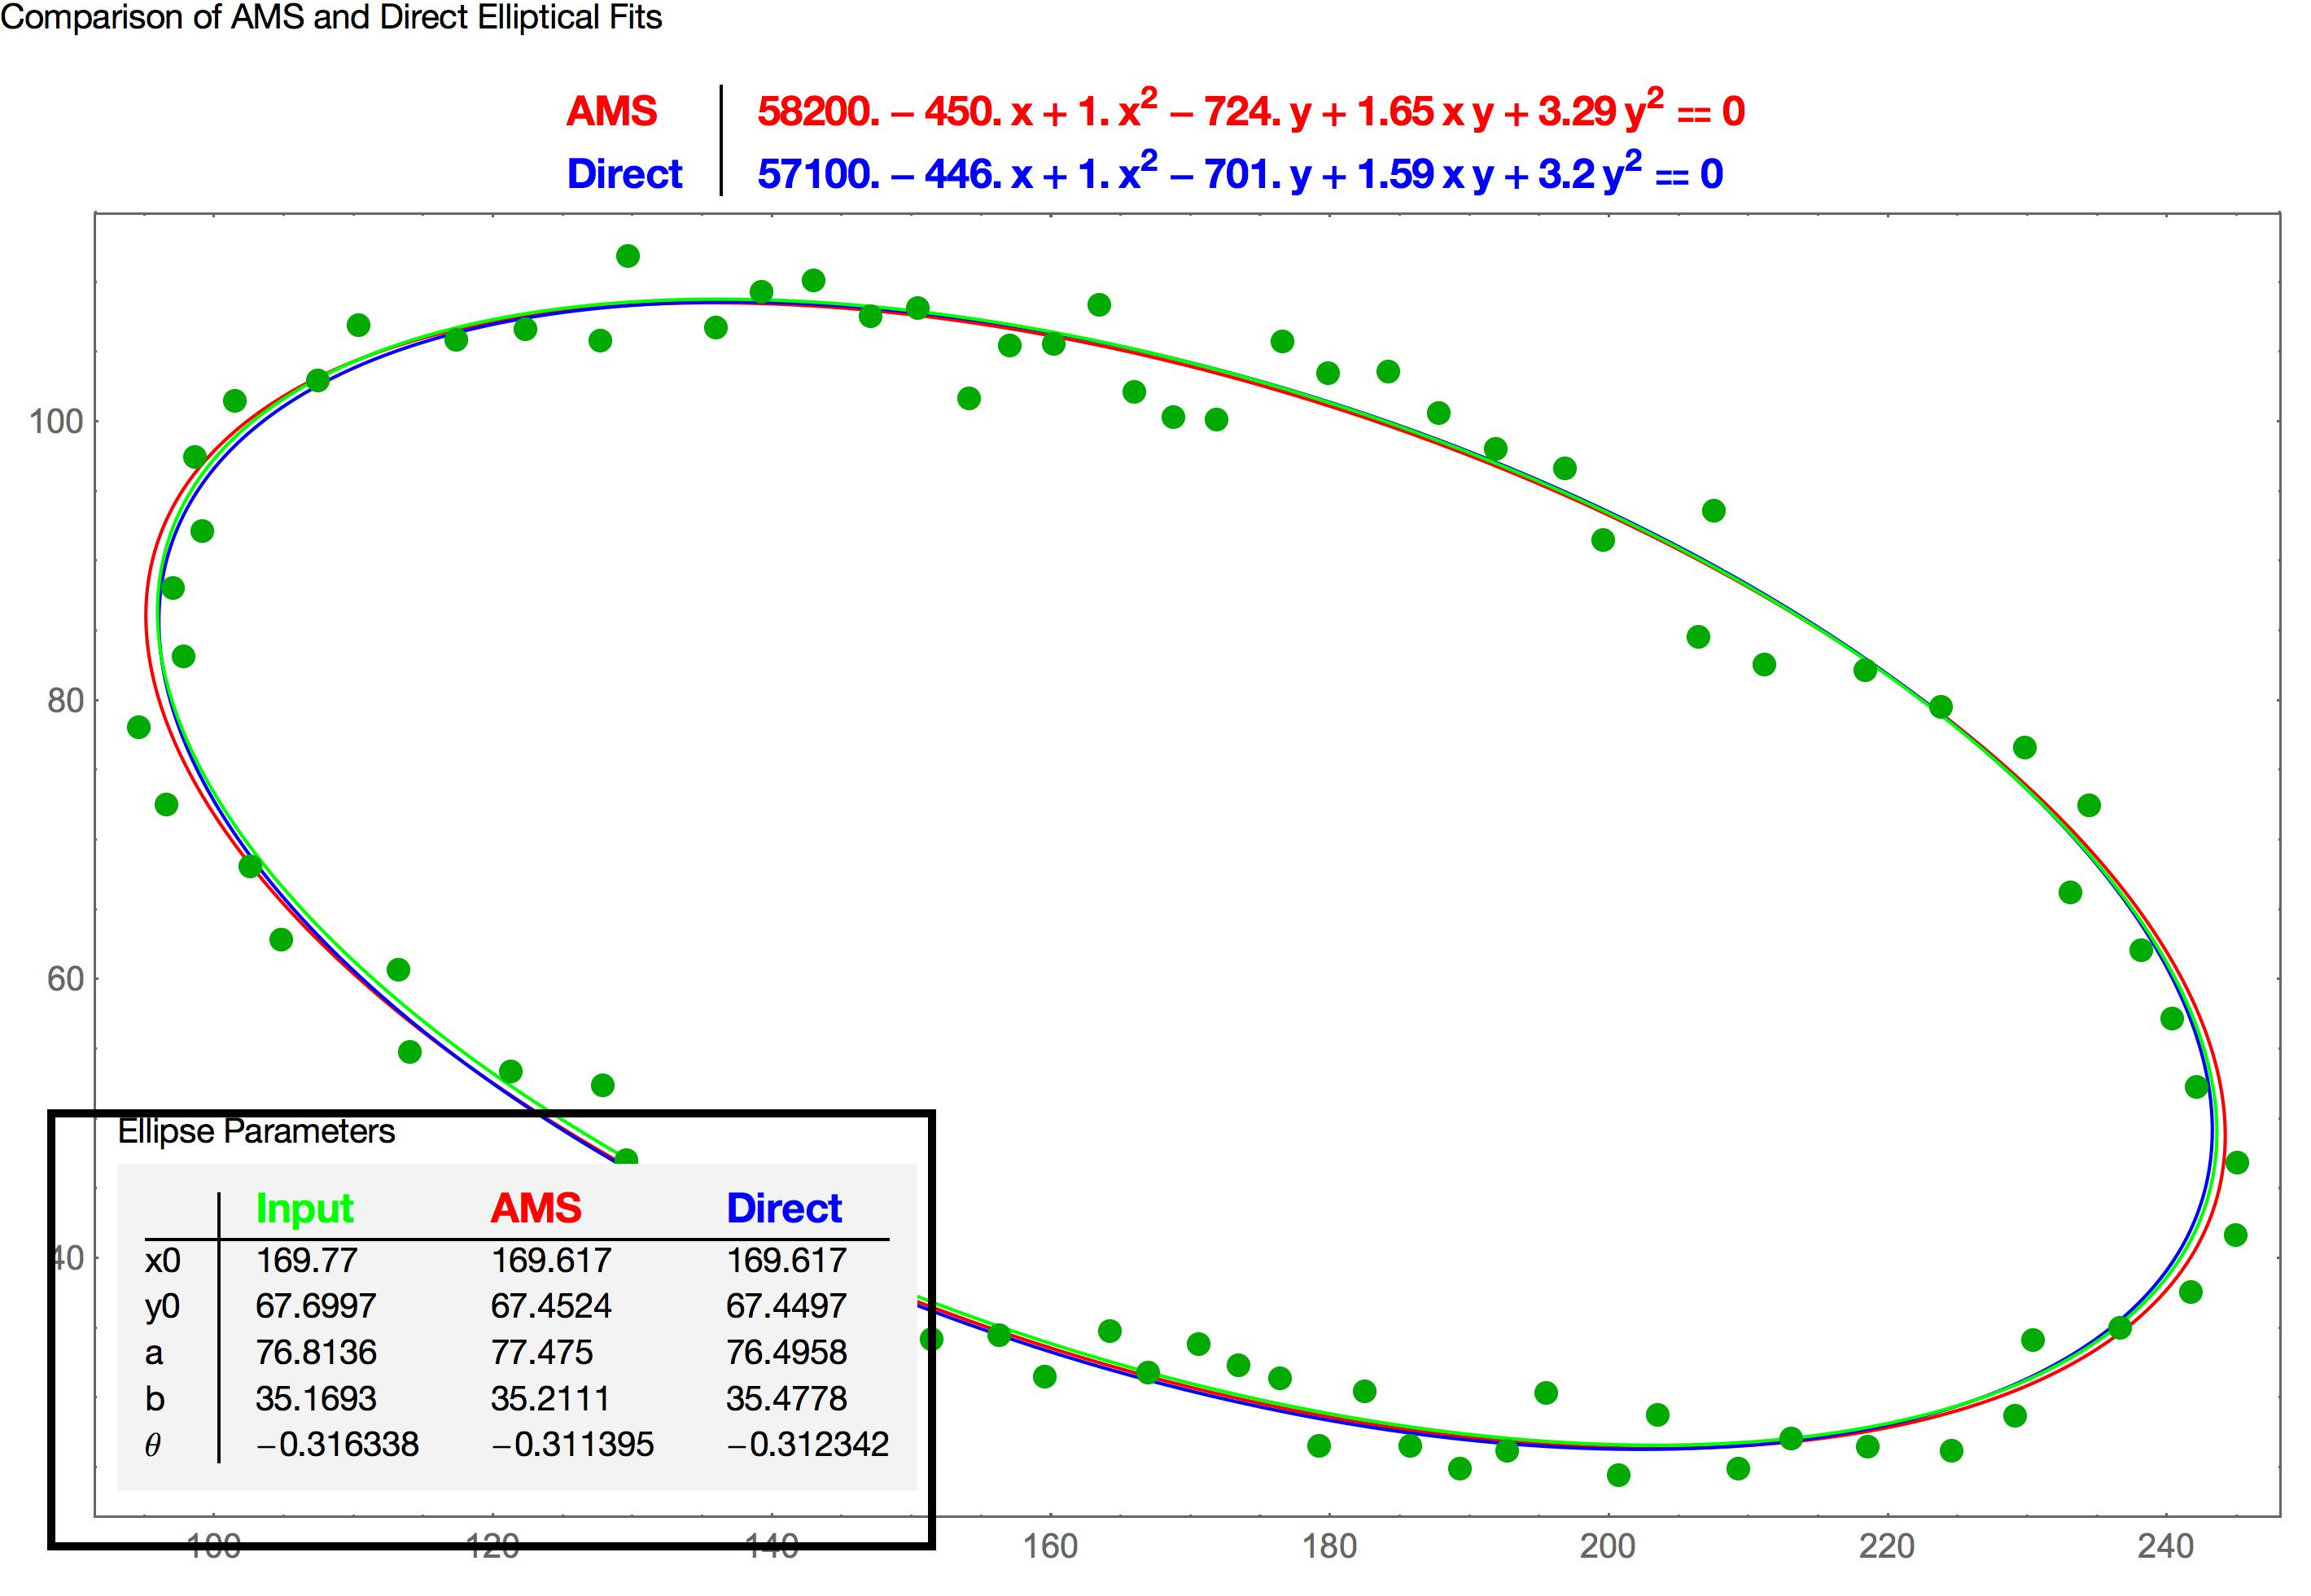
\includegraphics[width=0.98\textwidth]{Chapter4/Figs/EllipticalFitTestFull.jpg}
\label{fig:EllipseFitTestFull}}
\qquad
\subfloat[The AMS method sometimes produces a hyperbolic fit.][The AMS method sometimes produces a hyperbolic fit whilst the direct method always produces an ellipse]{
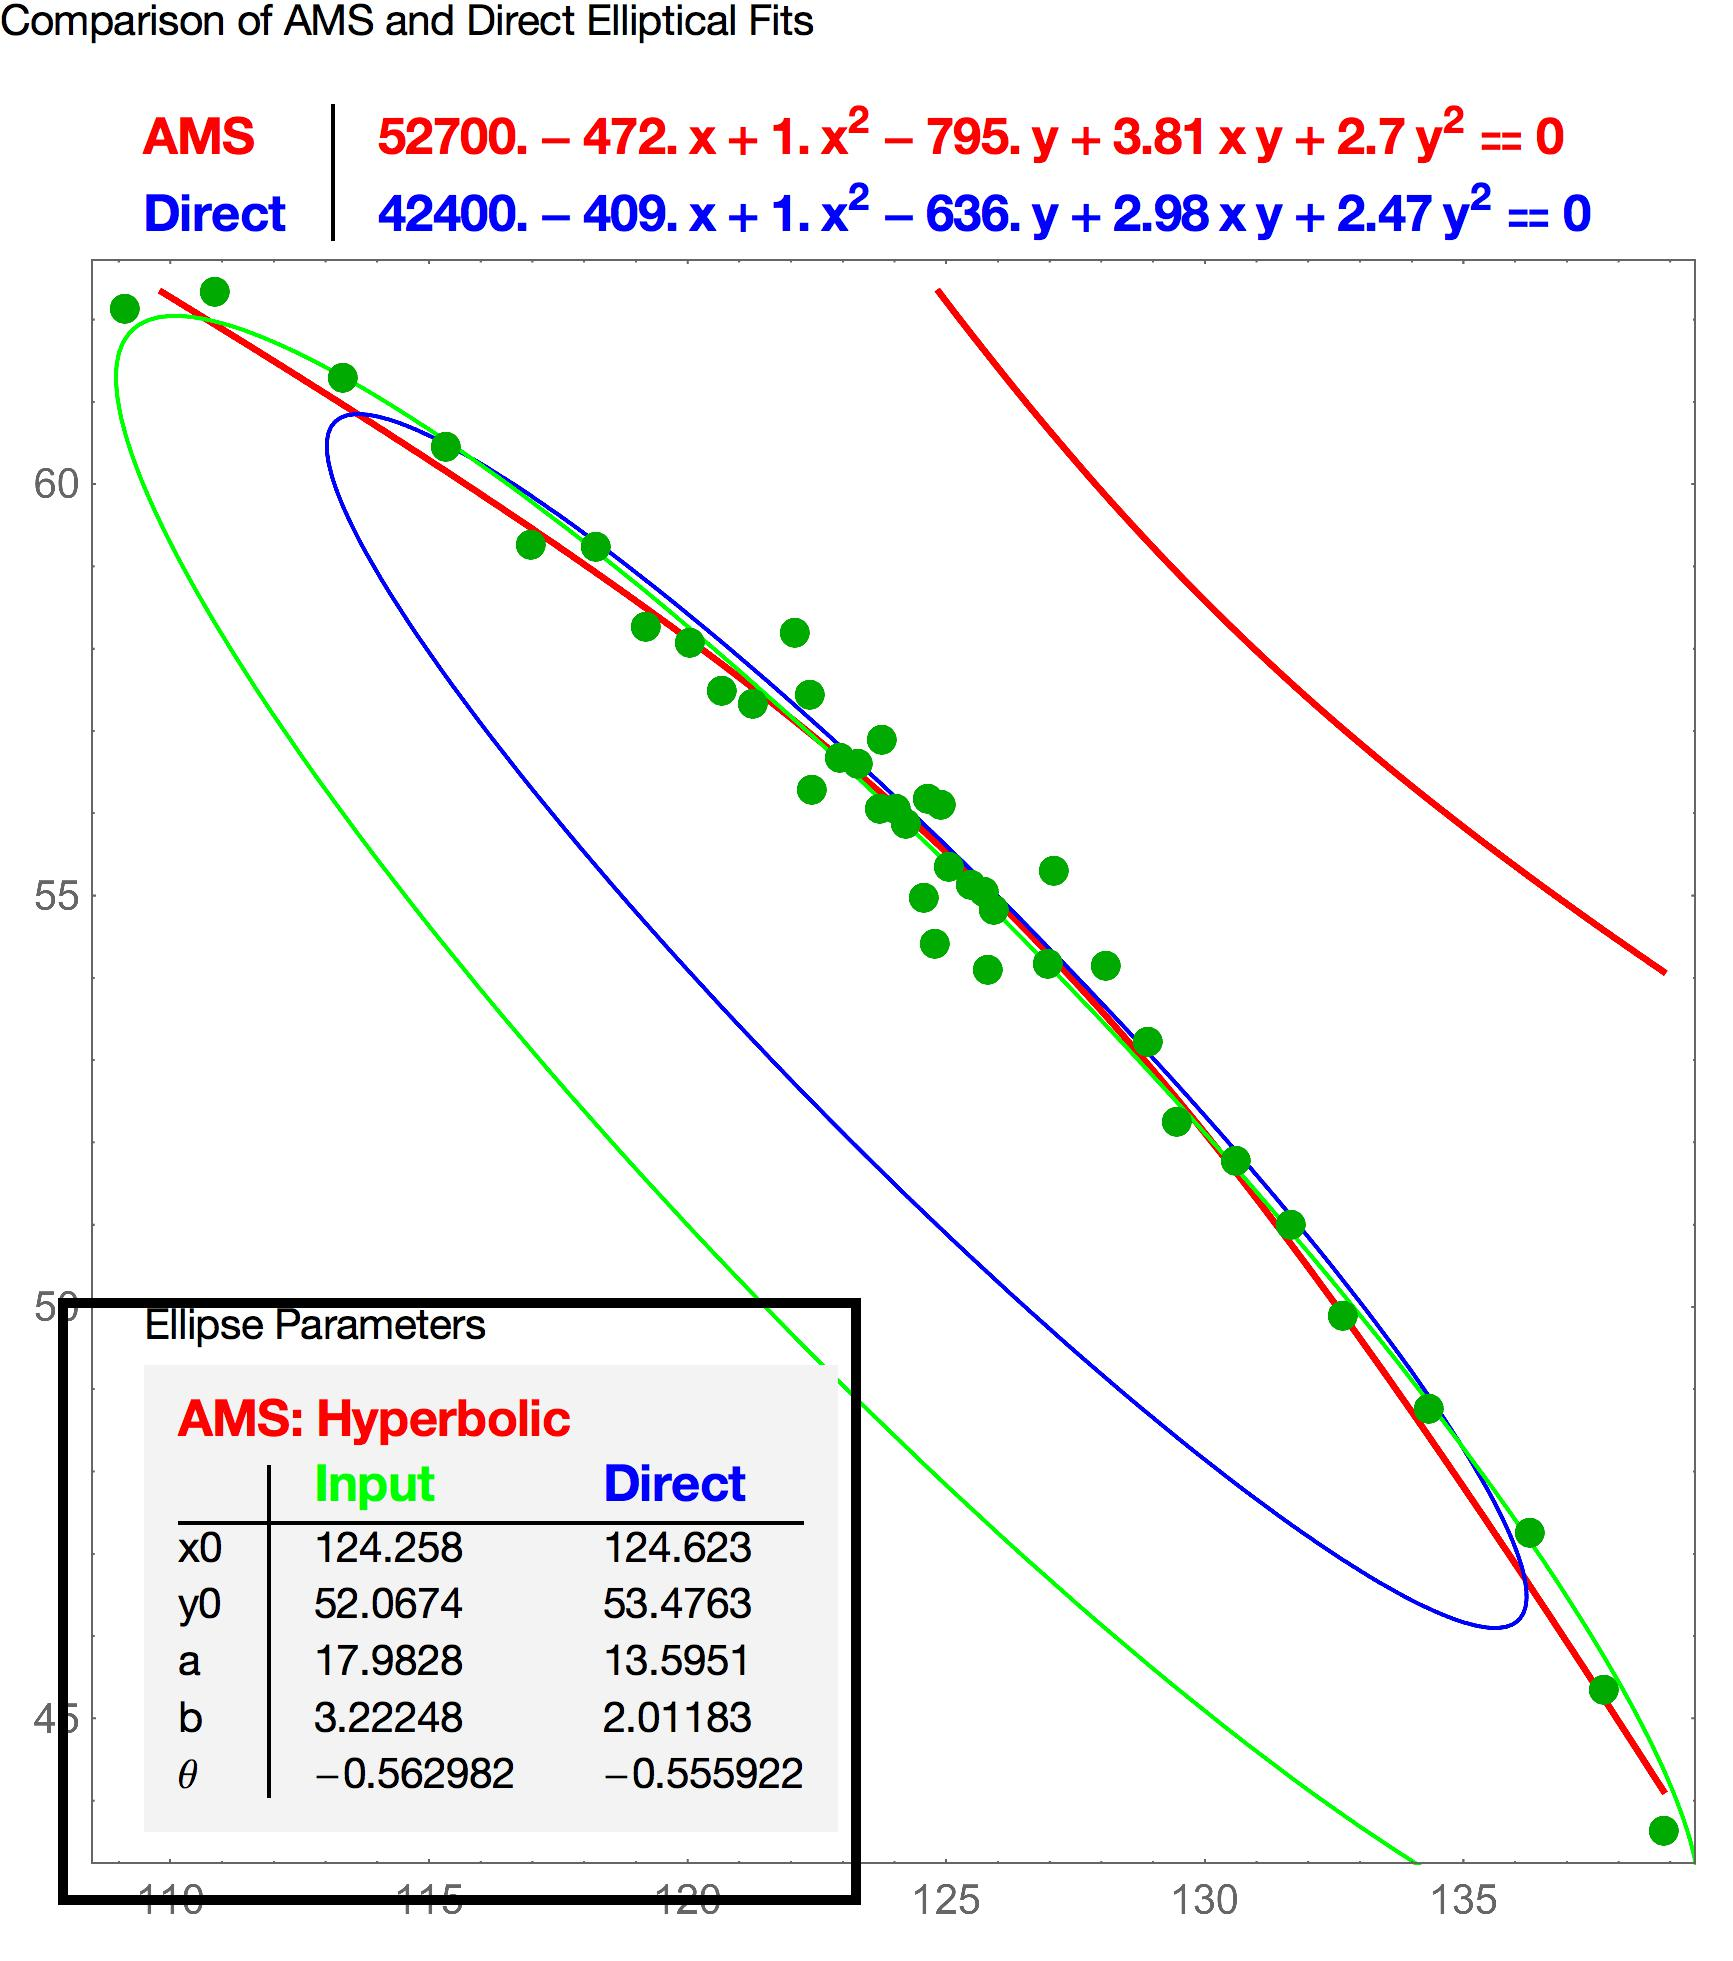
\includegraphics[width=0.47\textwidth]{Chapter4/Figs/EllipticalFitTest_Hyperbolic.jpg}
\label{fig:EllipseFitTestHalfHyperbolic}}
\quad
\subfloat[Comparison of the AMS and Direct ellipse fit methods for a half ellipse.][The AMS method better fits the extreme edge points in the data set resulting in the AMS method producing larger ellipses than the Direct method. The true ellipse is most often between the  two.]{
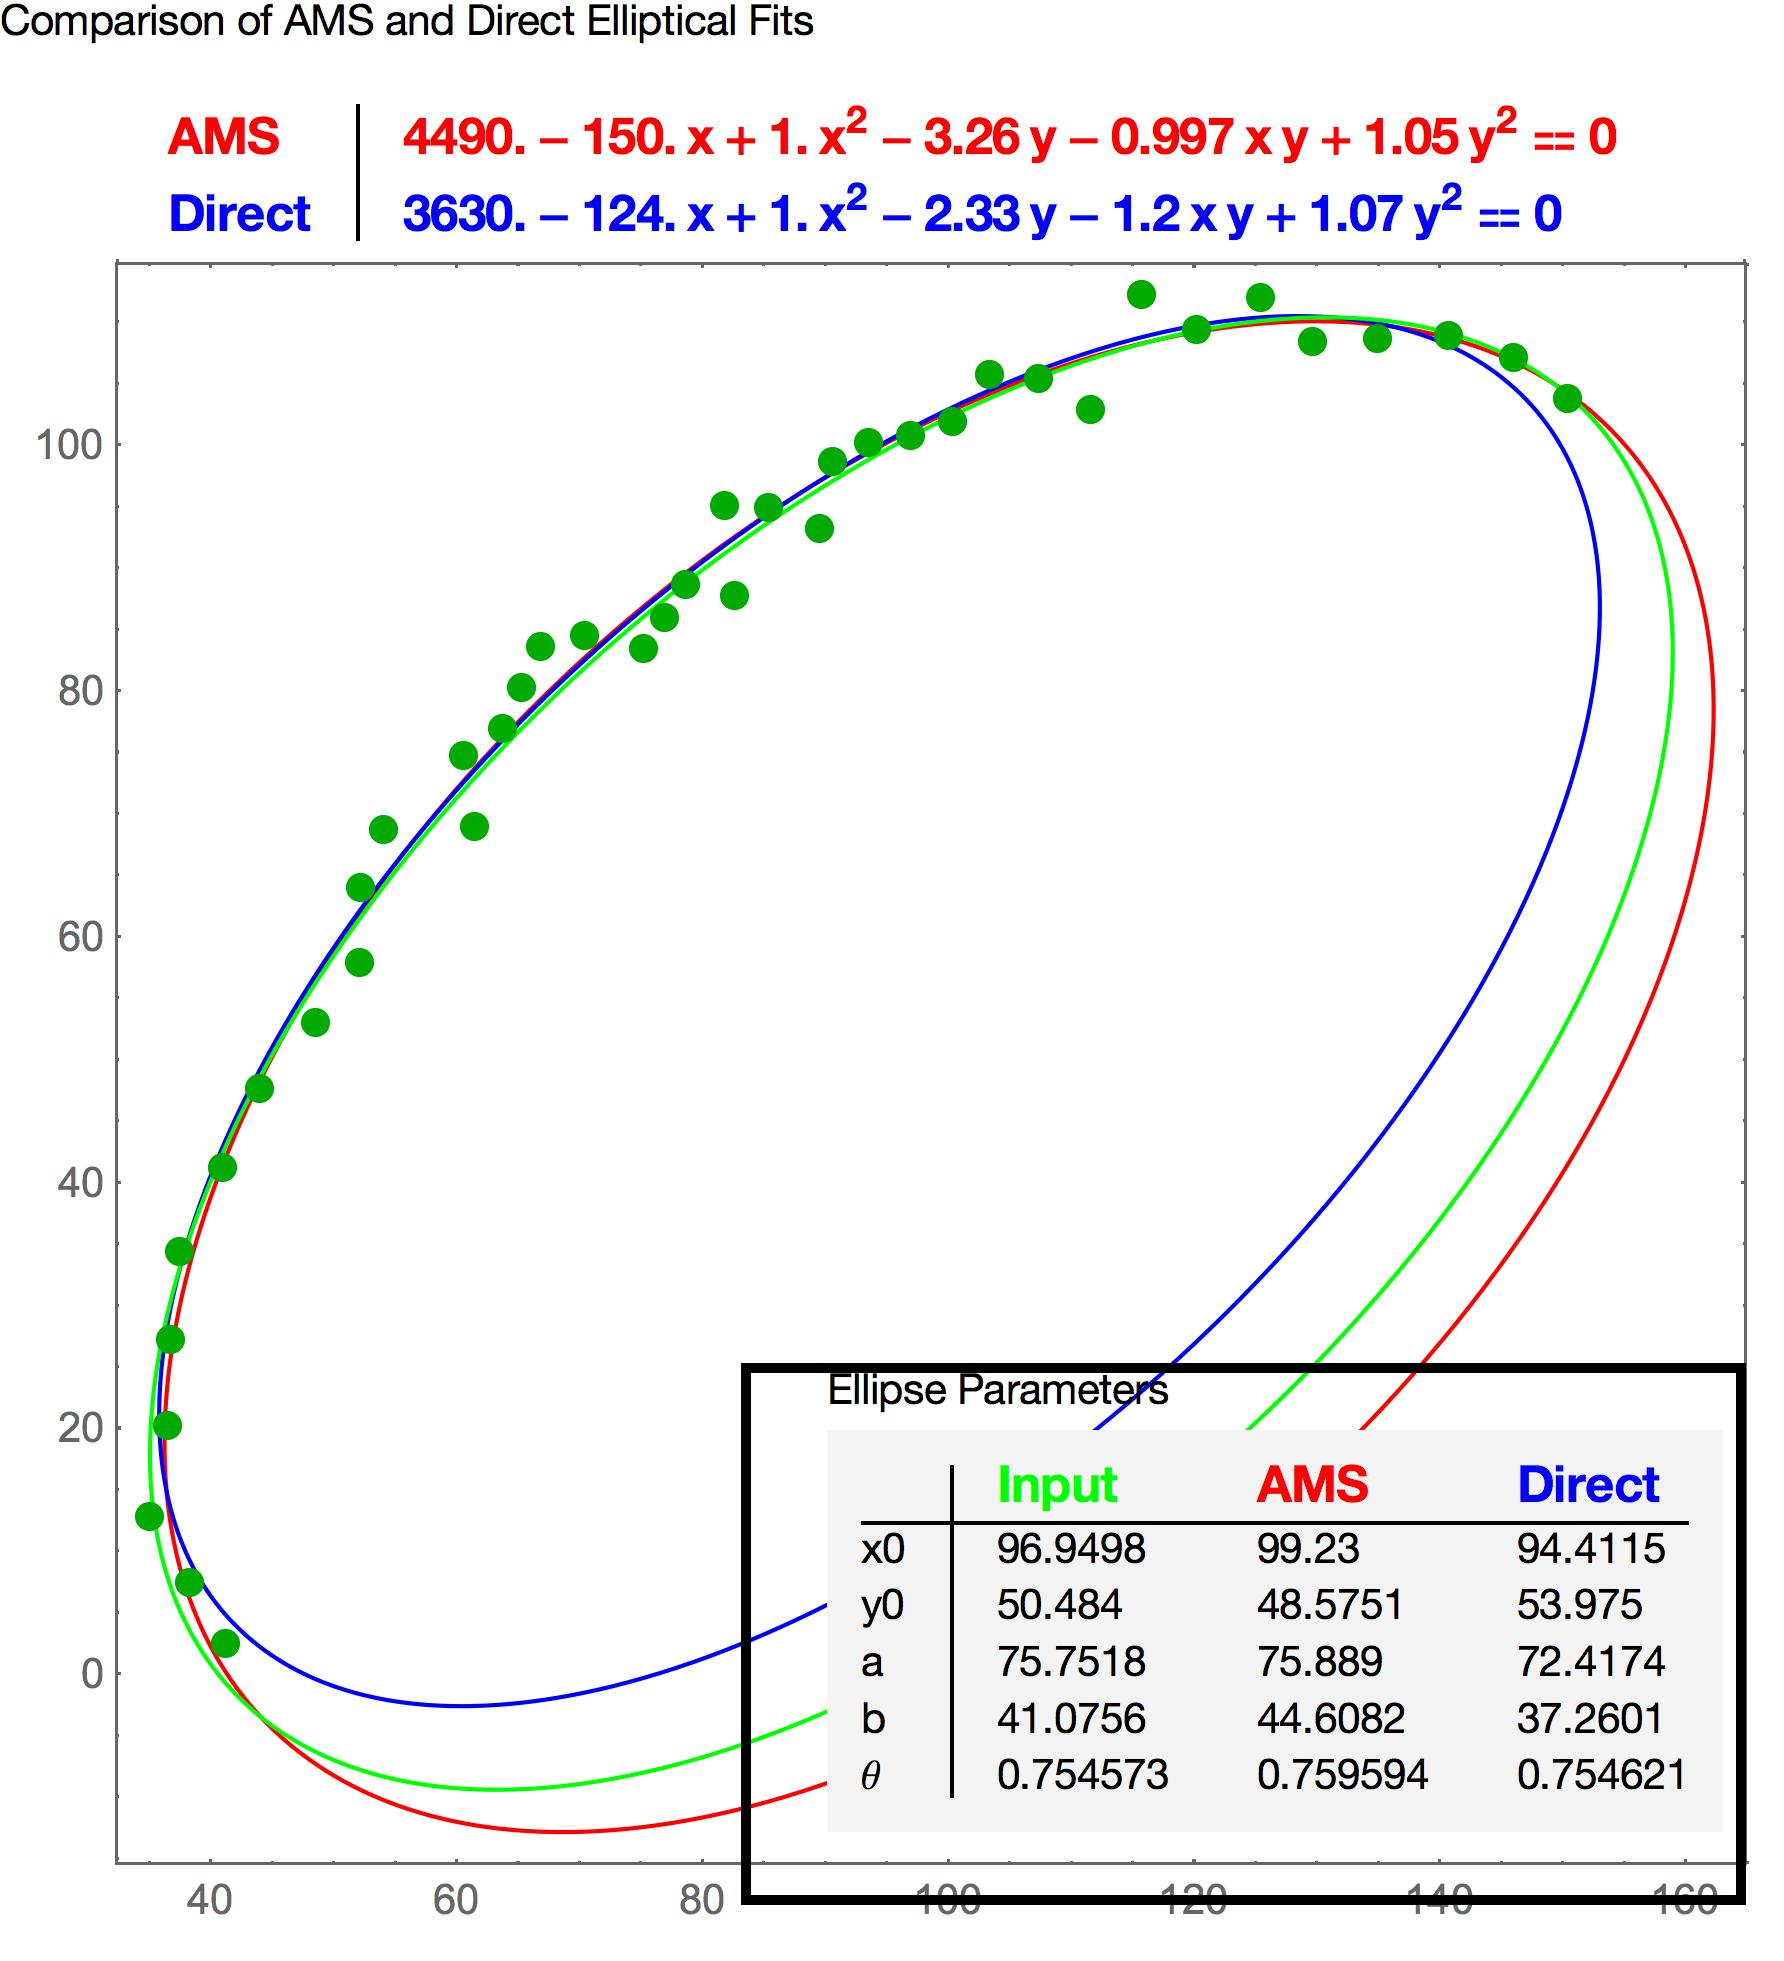
\includegraphics[width=0.47\textwidth]{Chapter4/Figs/EllipticalFitTest_DTA.jpg}
\label{fig:EllipseFitTestHalf}}
\caption{Comparison of the AMS and Direct ellipse fit methods.}
\label{fig:EllipseFitTest}
\end{figure}

\begin{equation*}
 A = \sqrt{\frac{1}{\mathbf{u}^T C \mathbf{u}}}  \mathbf{u}
\end{equation*}
The scaling factor guarantees that  $A^T C A =1$.

These methods were implemented in Mathematica for evaluation and in the OpenCV C++ code. Testing routines generated sample data with variable ellipse occlusion and noise around a randomly generated ellipse. The methods both produced good fits to complete ellipses and incomplete ellipses. The AMS method was slightly better at fitting the extreme ends of the ellipse generally producing a larger ellipse than the Direct method. Both methods accurately obtained the position and orientation. The AMS method occasionally produced a hyperbolic fit for very flat ellipses.


The largest computational effort in both methods is the determination of the $D^T D$ matrix, once found however both methods can be used at relatively little extra computational cost. All Ellipses between the two can be considered as valid fits also. This suggests a method which allows for extra information to be used to refine the fit. In the case of the finger model this is the orientation, distal width and position from the parallel line fit. The ellipse between the two fits which most closely matches the extra information is chosen as the best fit.

\subsection{The 'Isoscelian Trapezian' Fit}\label{sec:TrapezianFit}

Given three sets of points corresponding to the top, middle and bottom of a isosceles trapezium which is oriented so that the parallel sides are on the left and right a fit can be found as follows.

\begin{enumerate}
\item A straight line fit to the midpoints is found giving start and end points along with an orientation.
\item The points are translated and rotated so that the start point is at the origin and the end point is on the x axis.
\item The bottom points are reflected about the x axis.
\item A single straight line is fitted to the top and reflected bottom points together.
\item Four points describing the trapezium are found and returned along with the orientation and position in the original coordinates.
\end{enumerate}

\section{Fingertip Model}\label{sec:FingertipModel}

We need an appropriate finger model so we can accurately align points on the fingertip between successive images in the video stream. We need to do this because otherwise, any difference between the frames will be overwhelmed by physical movement of the digit rather than movement of the blood inside the digit. For this reason, we target the most stable portion of the finger: the nail.

A digit has two joints and three segments: the distal, the middle, and the proximal. Each segment is roughly approximated by a rectangle, and the length of each section approximately following a 2-3-5 ratio, with lengths counting from distal to proximal, and where 1 is the $\frac{3}{4}$ width of the middle segment. Each digit also has a roughly circular feature in the nail close to the tip of the distal segment. Our finger model then comprises of the lengths and widths of each segment, the positions of the joints (i.e. the knuckles) between each segment, the position of the tip, and a position in the model marking the point at which the digit goes out of frame. 

<Now, draw the thing, and show the initial guesses, and where the center is, etc.> 

Given the width of the middle segment, we can then have an initial guess that the length of the distal segment is 1.5 times the initial width, the middle is 2.25 times that, and the proximal is 3.75 times that. Additionally, the center of the nail feature is not in the center of the distal segment, but a half unit (in our model unit) away from the tip. The model can be laid out in units relative to the middle section.
\subsection{The Finger Shape Detection Algorithm}\label{sec:FingerShapeDetectionAlgorithm}

\subsubsection{Scale Space}\label{sec:ScaleSpace}
The images captured with the iPhone camera are extremely large, and so for the development of the algorithm, we define three scale spaces: one is the original image; two is an image size which represents the tip of the finger regardless of the distance of the camera from the finger, i.e. a scale relative to the width of the finger in the frame of the camera; three is a small image size for tracking the finger where it's freely roaming in the camera's view. We want these images to be formed without the need for resampling. For that reason, we restrict the choice of image sizes to those which are integer factors of the image dimensions. This is done by finding the integer factors of the original image dimensions and then selecting from those factors to scale the image. It should be noted that, to simplify point correspondences, the integer scaling from the small to medium scales is also kept.

\subsubsection{Finding the Frame Orientation}\label{sec:FindingTheFrameOrientation}
It is assumed we will not be using severed fingers, and so we know that the finger must exit the camera frame; the first step of the algorithm is then to detect which of the four edges the finger is entering from. This is done simply by finding the longest on-object path running along the frame sides. So, the algorithm stars by looking down the pixels on a frame side; when it locates a high-trinary value, it uses the Hurdle method to find the longest path in that direction starting from that point. It continues around all four sides; the longest path found by the Hurdle algorithm is assumed to correspond to the finger entering the frame. From this, we set a frame orientation, which is the angle necessary to rotate the image such that the finger will be entering the frame from the left, and we set a direction vector pointing inwards from the frame edge found.

\subsubsection{Finding the End of the Finger Shape}\label{sec:FindingTheEndOfTheFingerShape}
Taking the longest Hurdle path on the frame edge found above, we take the middle point on that path and start a "Run-Reach" algorithm in the direction found previously from that point. The Run-Reach algorithm proceeds as follows:

It finds a Hurdle path in the primary direction, i.e. perpendicularly away from the frame edge. At the end of the Hurdle path, it finds the Hurdle paths in the two perpendicular directions to its primary direction, i.e. parallel to the frame edge. It then finds the midpoint between the ends of the Hurdle path, and then uses that to start a new Hurdle path in its primary direction. The algorithm continues in this way until the end of the finger is found.

\begin{figure}[h!]
  \centering
    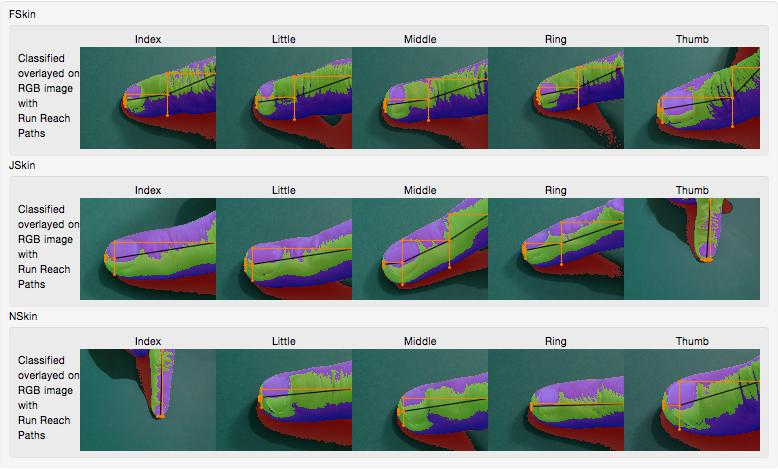
\includegraphics[width=0.95\textwidth]{Chapter4/Figs/FindingTheTip.jpg}
    \caption{Finding the End of the Finger Shape}\label{fig:FindingTheTip}
\end{figure}



\subsubsection{Filament Fill the Finger}\label{sec:FilamentFillTheFinger}
The center points found by the Run-Reach method above form a path on the finger. This is the path given to the Filament Fill method described previously. We now have a set of edge points on the digit. These edge points also have a top and bottom correspondence which, although they're not perpendicularly-opposite points on the finger, they do allow for a midpoint on the digit to be found. This can be seen in Figure~\ref{fig:FillamentFill}.

\subsubsection{Exclude Secondary Frame Edge Points and Fingertip Points }\label{sec:ExcludeSecondaryFrameEdgePointsAndFingertipPoints}
We need to exclude from the calculation of the midpoints on the digit values which are near the tip, and values which touch a second frame edge. This is because values toward the tip --- given that the finger is not necessarily perfectly horizontally-aligned --- give unreliable midpoint values because the Run-Reach path corresponds to shorter and shorter chords on a circle. Values which touch a second edge are, more likely than not, do not correspond to the edge of the digit, but are simply where the digit exits the frame. (For example, JSkin Middle in Figure \ref{fig:ExcludedEdgePointsAndMidlineFit}.)

\begin{figure}[h!]
  \centering
    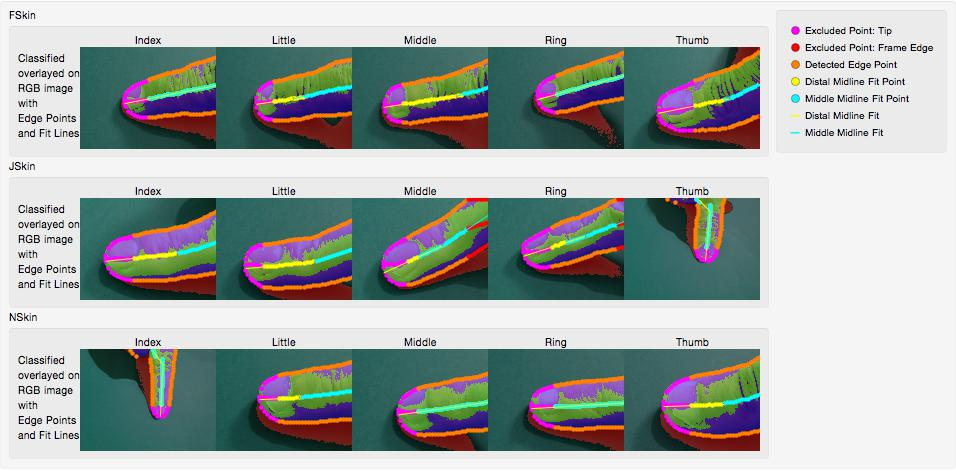
\includegraphics[width=0.95\textwidth]{Chapter4/Figs/ExcludedEdgePointsAndMidlineFit.jpg}
    \caption{Excluded Secondary Frame Edge Points and Fingertip Points, with the fit to the midline points returned by the Kink Fit algorithm.}\label{fig:ExcludedEdgePointsAndMidlineFit}
\end{figure}

To estimate which pairs of edge points corresponds to points on the tip, the algorithm finds the length of the Hurdle path for all corresponding bottom-edge to top-edge points. These values are then sorted into ascending order, and the lowest quarter and highest quarter are discarded, and the mean is taken of the remaining values. This ensures that the average is not affected by extreme values. This method is called the "Mean Median." Values which deviate significantly from this average are regarded to be outliers, or values on the tip. The tolerance is determined by the algorithm by looking at the difference at the low and high ends of the $50\%$ range.

\subsubsection{Kink Fit to the Finger}\label{sec:KinkFitToTheFinger}
We now have a set of reliable points at the midpoint of the finger. Because the finger is articulated, it is reasonable to assume that it may well be bent. We're interested in the action of the finger being pressed on a surface --- as a result. the finger is expected to be articulated at the distal-middle joint, but is otherwise straight. We wish to fit a function which consists of two straight-line segments to the set of reliable middle points. The fit was found using the Kink Fit algorithm described in subsection \ref{sec:KinkFitMethod}.

The Kink Fit algorithm as written takes a set of points where the first component is assumed to be the independent variable and the second component to be the dependent variable. However, because we haven't assumed that the finger comes into the frame from any particular direction, this can be problematic if, say, the finger comes through from the top or bottom of the frame, then the components would be in the wrong order for the Kink Fit algorithm to work. This is easily rectified by simply rotating the points into a standard orientation as if the finger is coming in from the left side of the frame. The computational effort in doing this is minimal because the number of points is small; we're not rotating the entire image, we're merely rotating a set of midline points, performing the Kink Fit algorithm, which returns a set of three points, which can then be rotated back to the original orientation.

In practice, however, the Kink Fit algorithm accepts the full set of midline points and a vector of pointers to the reliable values within that set. This allows the Kink Fit algorithm to extend out the end points of the line to the edges of the digit. Were this not the case, the end points returned would lie somewhere within the digit corresponding with the first and last reliable midline points. The result can be seen in Figure \ref{fig:ExcludedEdgePointsAndMidlineFit}.

\subsubsection{Parallel Lines Fit}\label{sec:ParallelLinesFit}
Our model of a finger assumes that the edges are parallel to each other. Since we have a line which runs through the center of the finger, we can now calculate the distance of the edge points to that line. These distances can be classified as good edge points if they're parallel to the central line. Whether they are parallel is determined by finding the Mean Median distance from the central line to the edge points using a $50\%$ interval in the distal portion, because it is expected that up to half the points may be in the distal segment, maybe on the tip, and a $75\%$ confidence interval in the middle segment, because we expect fewer than $\frac{1}{4}$ of the edge points to be anomalies. The points are then classified as good if they are of Mean Median distance from the central line. It should be noted that we consider both the top and bottom edges when calculating the Mean Median distance. This technique successfully removes anomalies which are not parallel to the central line.

There is one final step: the points which are classified as good edge points are used to find a linear fit which is parallel to the central line. Finally, the width of the distal and the middle segments is calculated by finding the distance between these parallel lines. This can be seen in Figure \ref{fig:ParallelFit}.

\begin{figure}[h!]
  \centering
    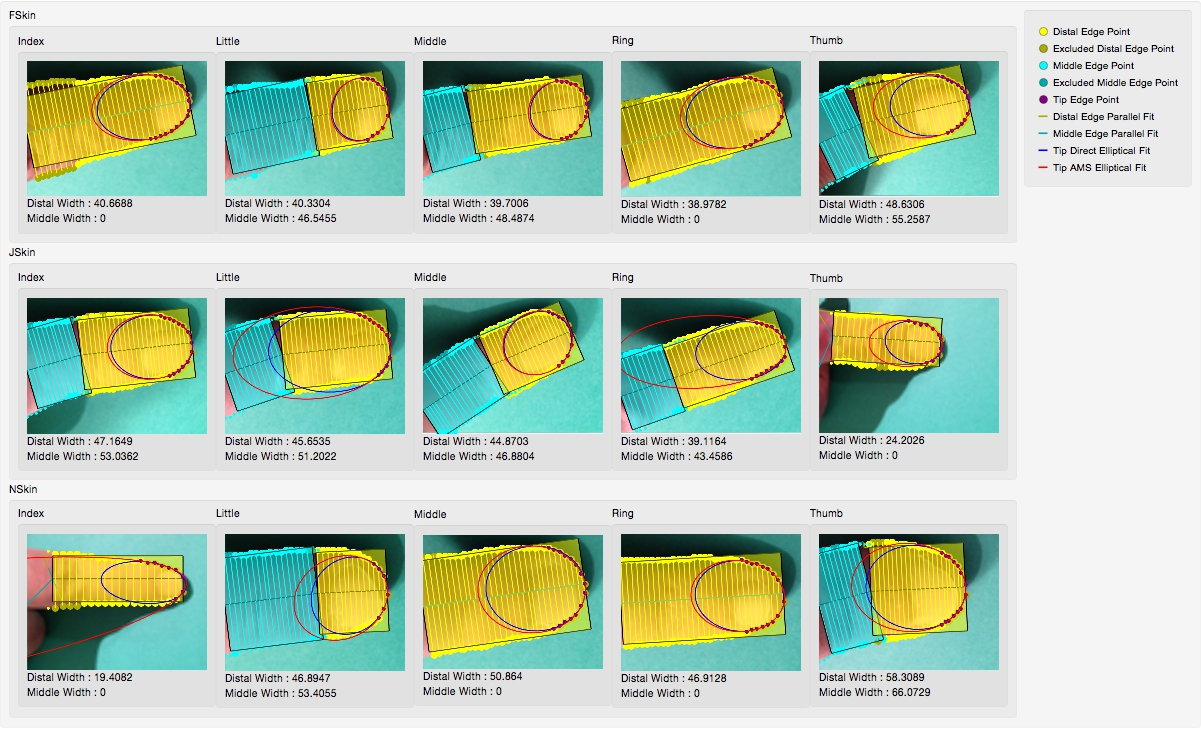
\includegraphics[width=0.95\textwidth]{Chapter4/Figs/ParallelFit.jpg}
    \caption{Initial shape-fitting stage, with the Kink Fit, midline, and Parallel Edge fit, with AMS and Direct elliptical fits to the tip.}\label{fig:ParallelFit}
\end{figure}

\subsubsection{Set the Scale Space}\label{sec:SetTheScaleSpace}
We wish to set the mid-scale such that the number of pixels across the distal segment is close to a chosen target value. As mentioned in the scale space subsection \ref{sec:ScaleSpace} we are restricting the choice of scales to integer factors of the original and integer multiples of the small scale. For the iPhone images the factors are:
\begin{align}
scale &= 2^{-i} 3^{-j} 17^{-k}  & i &\in \{0,1,2,3,4\} 
&  j &\in \{0, 1\} 
& k &\in \{0, 1\}
\end{align}

The small scale space is made using the largest number of small factors as possible to achieve the desired image size. This gives the greatest flexibility in scaling the mid-size.
\begin{table}[h]
\centering
\begin{tabular}{|cc|cc|c|c|c|c|c|l|}
\cline{5-10}
\multicolumn{3}{c}{ }  & & $0$ & $1$ & $2$ & $3$ & $4$ & i\\
\cline{1-10}
k & $k_{scale}$ &j & $j_{scale}$ & $1$ & $\frac{1}{2}$ & $\frac{1}{4}$ & $\frac{1}{8}$ & $\frac{1}{16}$ & $i_{scale}$\\
  \hline \hline
\multirow{4}{*}{$0$} & \multirow{4}{*}{$1$} & \multirow{2}{*}{$0$} & \multirow{2}{*}{$1$} & 
 2448 & 1224  &  612  & 306  & 153 & w \\
  &  &  & & 
  3264  & 1632  & 816  & 408  & 204  & h\\
  \cline{3-10}
 &  & \multirow{2}{*}{$1$} & \multirow{2}{*}{$\frac{1}{3}$} & 
 816  & 408  & 204  & 102  & 51  & w \\
 &  &  & & 
  1088  & 544   & 272  & 136  & 68  & h \\
\hline 
  \hline
\multirow{4}{*}{1} & \multirow{4}{*}{ $\frac{1}{17}$ } & \multirow{2}{*}{$0$} & \multirow{2}{*}{$1$} & 
 144  & 72  & 36  & 18  & 9 & w \\
 &  & & & 
  192  & 96  & 48  & 24  & 12  & h \\
    \cline{3-10}
 &  &  \multirow{2}{*}{$1$} & \multirow{2}{*}{$\frac{1}{3}$} & 
 48  & 24   & 12  & 6   & 3 & w \\
   &  &   & & 
  64  & 32  & 16  & 8  & 4  & h \\
\hline 
\end{tabular}
\caption{The image pixel dimensions for all possible integer factor scalings.}
\end{table}

So for a chosen small scale $S_s = 2^{-3} 3^{-1}$, a distal width in the small scale $w$ and a minimum distal width in the medium scale $w_m$. 
Finding  $i_m$ and $j_m$ which minimise $i_m + \frac{\log(3)}{\log(2)} j_m$  and which satisfy  $2^{-i_m} 3^{-j_m} - \lceil \frac{w_m}{w} \rceil \ge 0$, $i_m\le i_s$ and $j_m \le j_s$ determines the medium scale space.

\subsubsection{Elliptical Fit to the Tip}\label{sec:EllipticalFitToTheTip}

We wish to fit an ellipse to the points found at the tip of the finger. We've chosen an ellipse because we are assuming that the tip is symmetrical about the mid-line fit, and that the extreme edges are parallel to the mid-line. Using an elliptical fit outlined in section \ref{sec:EllipticalFitMethod}, then, will exclude points which do not agree with these assumptions, thereby eliminating anomalies.

However, it should be noted that the points provided by the parallel lines fit (Fig \ref{fig:ParallelFit}) are not good enough to determine which parts on the curved tip of the finger, which we're approximating as roughly elliptical, due to the tapering of the distal segment of the finger towards the tip, as well as the alignment of the digit in the frame.

\subsubsection{Modeling the Fingertip}\label{sec:ModellingTheFingertip}
Having determined a measure of the width of the distal portion of the fingertip allows for a more robust model of the fingertip to be determined. This is because the measurement of the distal width is far more reliable than the distal length which has so far been determined, as the distal length has been found by evaluating where the "kink" of the midline points lies. For example, if the distal joint is unflexed, the knuckle portion will be overlooked entirely, as seen in Figure \ref{fig:ParallelFit}. It turns out that the anatomical ratios (Section \ref{sec:FingertipModel}) are a far more reliable method of determining the distal length.

From the kink fit, we have a midline, which is specified by three points. We now determine two points on this line, which are $\frac{1}{2}$ the distal width ($d1$) and $1\frac{1}{2}$ the distal width from the tip ($d2$). So the midline point that lies between the two points can now be taken to correspond to the straight-edged section of the distal portion of the finger. These points are passed to the Trapezian Fit method (\ref{sec:TrapezianFit}), and the points which lie between the tip and the point half the distal width from the tip are passed to the Elliptical Fit (\ref{sec:EllipticalFitMethod}). The ellipse is adjusted to correspond with the two near vertices of the Trapezian; the result can be seen in Figure <put figure here>.

\begin{itemize}
\item \textbf{Determining $d1$ and $d2$} --- we have a line which is given as two points; one somewhere on the digit, and the other at the tip. If the finger were straight in the frame, then $d1$ and $d2$ are easily found by finding the points on that line. However, the fact that the digit can be presented at an angle means that the edge points vertically above and below the point on the midline may include part of the curved tip. This has the effect of making these midpoints diverge from the midline of the digit. This can be corrected by adjusting with half the gradient of the midline to the ratios. \begin{equation}distance \:on \:line = (\frac{1}{2} + \frac{1}{2}\delta\:mid)w\end{equation}.

\item \textbf{A New Midline Fit} --- we take the set of midline points, extract the subset which lies between $d1$ and $d2$, and then apply a straight line fit to these points.

\item \textbf{Determine an Origin and Orientation} --- the origin is the fit evaluated at the x component of $d2$, and we determine an orientation $\theta$, which is $\arctan$ the gradient of the linear model.

\item \textbf{Determine the Neutral Coordinates} --- We move all the points --- the top and bottom edges, and the midline points --- and we translate to the new origin. Then, we rotate by $-\theta$. This we call the "neutral co-ordinates", as the tip is aligned with its midaxis lying on the x axis. These points are separated at one distal width from the tip; a Trapezian fit is applied to one set of points, and an Elliptical fit is applied to the other. As a refinement to this, although the linear fit is applied as in the Trapezian section, the algorithm then looks at the points beyond and before the one distal width region; if they're consistent with the fit, then they are considered still part of the straight edge. The Elliptical fit is applied as discussed previously. 

\item \textbf{Fitting the Shapes} --- The comparison between the methods is done by looking at the distance from the front two points on the trapezian to the edge of the ellipse, and the best of these is chosen. Unfortunately, this is often not sufficient to make the ellipse join with the trapezian exactly because further on in the algorithm, these shapes will be used to perform a mask; we want to avoid introducing artifacts which could be interpreted as features. So, we wish to remove these discontinuous intersections between the ellipse and the trapezian. In order to do this, we choose three points on the Elliptical fit and the two front points of the trapezian, thereby making a set of five points, and we pass these through the direct Elliptical fit algorithm. It should be noted that five points is what is required to completely define an ellipse; there is one on the ellipse which will pass through five points.

\item \textbf{Finalizing the Model} --- The coordinates for the ellipse and the trapezian are adjusted so that the origin is at the center of the ellipse, and the ellipse has zero rotation. The reason for this is that it makes calculating the distance from the edges of the ellipse easier. So, now when we apply the model to the image, all that's required is a position --- which is the position of the center of the ellipse --- and an orientation about that position. 
\end{itemize}


\section{Putting it All Together}\label{sec:PuttingItAllTogether}

So far, we have said little about how we actually intend to detect a digit being pressed on a surface. Although a significant amount of discussion has been presented to do with the optimization --- at least in terms of the data types and the underlying maths --- mostly to do with the color space transform. We have said even less about the size of the images captured or the framerate at which the processing is required. These are important considerations for designing practical code, especially for application in a mobile device.

\subsection{Detecting a Finger Press}\label{sec:DetectingAFingerPress}

In the previous section, we presented several algorithms which perform steps in the task. However, we now need to put them together and fill in the gaps which link each important step together. Assumptions and simplifications which we have allowed ourselves in this work which is intended only to be a proof of concept rather than a fully-fledged application. To this end, we have decided to simplify the requirements and --- although there is no compelling reason why we could not use, say, convex hull and defects to detect the fingers, or even a full hand --- we're only going to consider the case where one digit is presented to the routine in a controlled environment:

The first step in the algorithm is to select a human and a camera. With this done --- using the same camera as will be used by the application --- we gather statistics for a particular individual's skin, trying to vary the lighting conditions so as to give us as representative a data set as possible. From this, a color space is designed and the relevant transforms and such are instantiated for that particular individual.

The next step is to collect the finger features and instantiate the feature detectors using the Canny-edge-based descriptor for each of the individuals' digits.

Now we start the application: it turns on the camera and waits for movement. After the movement starts, it continues to wait until that movement slows, which is the first indicator that a surface is being touched. Here we assume that we are trying to detect static presses, so no pressing and dragging is considered. We look at a higher resolution frame, process that frame into the skin color space for the individual in question. 

Now we perform our shape detector, which looks for a finger-shaped object, finds the tip, creates rectangular bounds for the tip, and then takes an even higher resolution frame. (But only for the tip of the potential finger.) This image --- cropped to the tip of the digit --- is then sent to the feature detecton algorithm, which then uses the Canny edge feature method previously described and attempts to identify the digit by applying the known descriptors for the individual's nail.

These steps are relatively slow, but --- once applied --- the algorithm now only tries to fit one feature descriptor and simply tracks the assumed small movement of the tip during a press. Due to the slow nature of these steps, it's required that the camera buffers a few frames after the motion stops, otherwise the finger press may miss the processing window. It is at this stage that the algorithm to detect the finger press really starts.

Now that the fingertip has been located, the algorithm crops the fingertip before forming the color space transform, which saves a significant amount of processing time. We now define a larger cropping region, and a tight cropping region. The larger of the two cropping regions is used initially to ensure that the entire tip of the digit is captured in subsequent frames, as this cropping region will not vary during the finger press detection stage of the algorithm. Inside the cropping region, a second rectangular region is defined, which is centered using the feature detection, ensuring that the frames are aligned with the true outline of the digit and not the outer pixels. Any change in the tighter frame will be due to the mechanical action on the digit changing its visual appearance.

The tightly-cropped region from each frame is held in as high a resolution as possible, and the absolute distance between each successive frame is calculated in this region. It was discovered that the color channel corresponds to the major axis of the 2D Gaussian fit to the chromatic space. It has been found that a finger press changes the chromatic values in the end of the digit sufficiently for this to register clearly in this region. For the purposes of this project, this difference is calculated and output as an image. However, for the actual application, all that is required is a measure of the size of the change in the chromatic space.

\begin{figure}[h!]
  \centering
    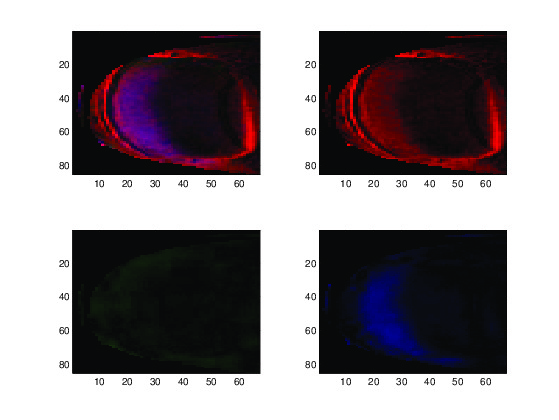
\includegraphics[width=0.90\textwidth]{Chapter4/Figs/jThumb_Final_Proof.jpg}
    \caption{The difference in the skin color space between successive frames during a finger press. (Or in this case, a thumb.)}\label{fig:FinalProof}
\end{figure}

The second indicator for a finger press was found around the center of the pad of the digit. The distance to the convex hull --- which outlines the edge of the digit in the frame --- was noted to move away from the centered reference point. This is because the nail does not significantly deform under mechanical stress, however the soft tissue underneath does. This provides a second level in the metric for detecting a digit press.

The algorithm now decides based on thresholds which could be trained, but in the present implementation were set manually, one on the chromatic difference in the feature region (i.e. the nail), and the second on the contour from the shape detection. The output of each combined to produce a sound, the idea being the harder you press, the louder the noise.

The final step is to detect when the digit starts moving again. Failure of the feature detector to re-align the small frame makes the algorithm start tracking motion again. It looks at the low-resolution frames and sees if significant movement is occurring in the larger frame. It should be noted that the algorithm does not process outside of the larger cropped region during the finger press detection phase.

\section{Skin Detection}\label{sec:SkinDetection}

With the image in the skin color space, skin detection is a significantly simplified problem; the average skin color is at the halfway point in both of the chromatic channels and the Gaussian distribution has already been applied, meaning that performing an elliptical thresholding in the normal color space is equivalent to a rectangular thresholding in the skin color space. The probability distribution can be obtained by combining the distributions in each chromatic channel. Because the thresholding levels in each channel are equivalent to the same points on the Gaussian, they can be straightforwardly combined, and then a single threshold used on the one resulting channel. This can be done by subtracting $\frac{1}{2}$ from both channels, squaring them, then adding them together.

The next step is to identify the skin. For the purposes of this project, we're searching for a skin-colored object of a specific shape: a finger that comes into the frame, presses down on a surface, then exits the frame. One of its properties is that it meets the edge of the frame, appearing as a rectangle with a rounded end which --- on occasion --- can appear slightly bent due to the viewing angle or pressure placed on the finger as it presses down on the surface. But there's a limit to how great that deflection can be in the image.

In order to find this shape, we begin by finding the contours in the binary probability image. This can be achieved by using the "findContours" method in OpenCV, which finds the contours and returns them as a vector of points. In the skin color space, finding the contours around the finger is very simple.

\begin{figure}[h!]
  \centering
      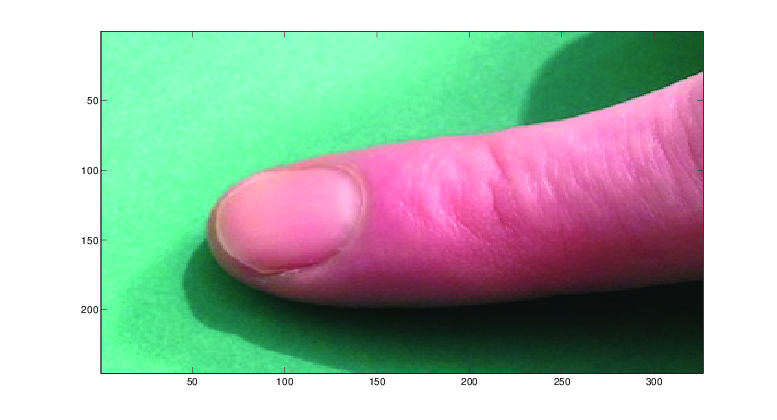
\includegraphics[width=0.45\textwidth]{Chapter4/Figs/imgJIndex1.jpg}
    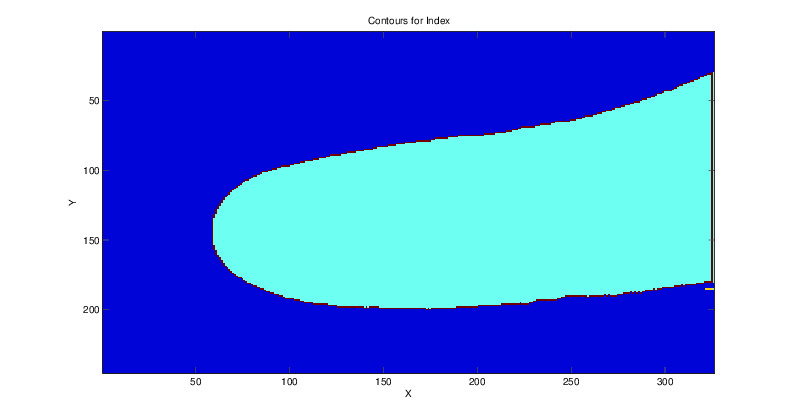
\includegraphics[width=0.45\textwidth]{Chapter4/Figs/indexContours.jpg}
    \caption{Finger contours in the probability image.}\label{fig:IndexContours}
\end{figure}

Once the contours have been identified, a rectangle is drawn around the finger using OpenCV's "rectangle" method, with the tip of the finger touching one of its sides. Next, lines are drawn along the sides of the finger using the "line" method, and a convex hull identifies the semicircular fingertip, again using an OpenCV method, in this case "convexHull." This produces a set of verteces which allow us to locate the fingernail, at which point we highlight it with a square drawn using the "rectangle" method once more. The fingernail image within this square is then sent to the edge detector method for further processing. (See Figure 2.17.)

It should be noted that --- in the finger images in Figure~\ref{fig:IndexContours} --- the finger is deformed slightly due to the application of pressure on a flat surface, as was discussed previously. This doesn't necessarily share the same orientation as the tip. This can be remedied by taking the portion of the image highlighted by the rectangle and performing the operation again, thereby producing a rectangle which is properly oriented with the fingertip.

Once the fingertip has been identified, its features are obtained using the SURF algorithm method provided by OpenCV's SURF class. An initial attempt was made to use the library functions in OpenCV, however the high resolution and the relative uniformity of the fingertip resulted in no stable feature points being automatically detected. The initial idea was to allow the automatic descriptor generator to use a set of aligned frames and the idea was to keep the features which were stable in time and space. (i.e. Present in every frame and in the same location.) This attempt was unsuccessful, so a bespoke method was designed instead.

\begin{figure}[h!]
  \centering
    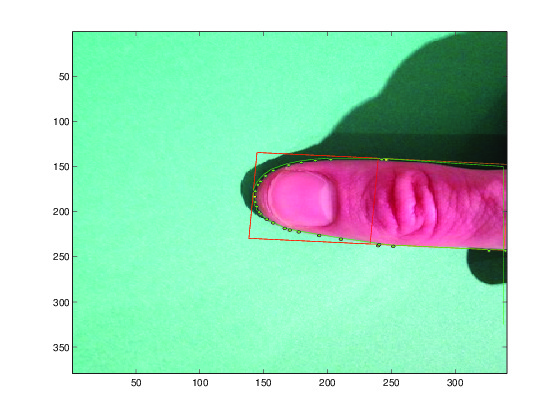
\includegraphics[width=\textwidth]{Chapter4/Figs/shapeDetection.jpg}\label{fig:shapeDetection}
    \caption{Shape detection in action.}
\end{figure}

\begin{figure}[h!]
  \centering
    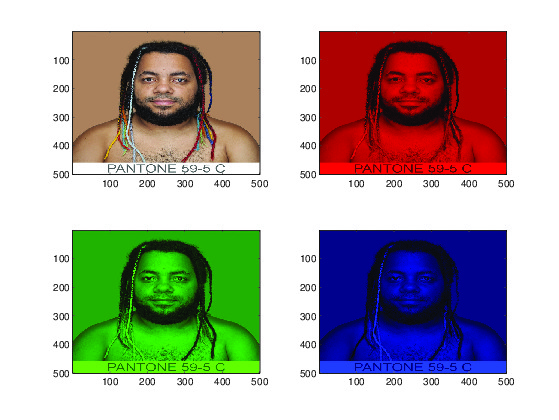
\includegraphics[width=\textwidth]{Chapter4/Figs/rainbowmanRGB.jpg}
    \caption{RGB channels.}
\end{figure}

\begin{figure}[h!]
  \centering
    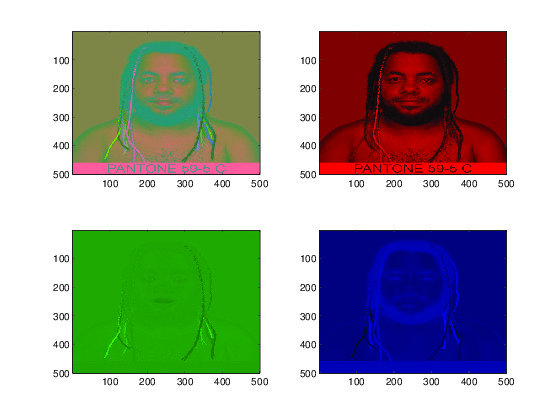
\includegraphics[width=\textwidth]{Chapter4/Figs/rainbowmanRotated.jpg}
    \caption{Rotated color space.}
\end{figure}

\begin{figure}[h!]
  \centering
    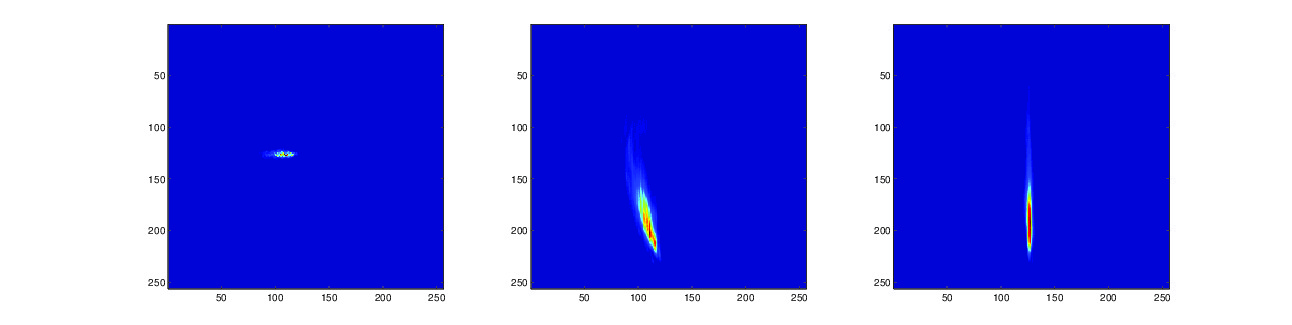
\includegraphics[width=\textwidth]{Chapter4/Figs/binsFinal2.jpg}
    \caption{Final bins.}
\end{figure}

\begin{figure}[h!]
  \centering
    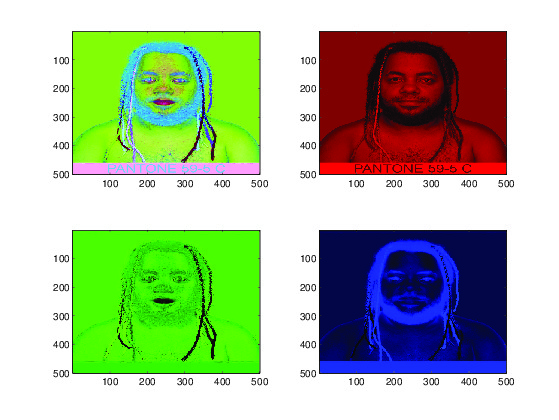
\includegraphics[width=\textwidth]{Chapter4/Figs/rainbowmanRotatedScaled.jpg}
    \caption{Rotated and scaled color space.}
\end{figure}
